\chapter{Experimental Verification}
An initial experimental proof of principle experiment was performed at the SACLA FEL.
The experiments consisted of three parts: First, reproducing XXX and imaging projection of the focal volume of the FEL by using metal foils as samples, performing a measurement of the K$\alpha$  fluorescence and an reconstruction in the small angle regime. Second, moving the a smaller length scale and try to image nanoparticles. And Third, leaving the small angle regime and record the fluoresccne of a single crystal and perform a reciprocal space reconstruction.
\section{Sample Preparation}
As an nanoparticle sample, spherical iron oxide nanoparticles where chosen. To improve the number of detected fluorescence photons per FEL shot, the decision was made to have many particles many for each shot within the focus. This ensures a higher number of fluorescence photons recorded and basically eliminates the possibility of having shots without any particles inside the focus. 

Magnetite Nanoparticles coated with Oleic Acid dispersed in Toluene were bought from NN-Labs, inhibited Methylmethacrylate (MMA) and Etyhlhexylmethacrylate (EHMA)  (Sigma Aldrich) were filtered using a prefilled column to remove the Inhibitor,  2,2-azo-bis-isobutyrylnitrile (AIBN) (Sigma Aldrich) was used as thermally activated radical initiator as received. Polystyrene (Sigma Aldrich, MW XXX) was used as received. As solvents, Methanol, Toluene and Chloroform were used.
\subsection{Nanoparticles in Polystyrene Matrix}
The nanoparticles were precipitated with Methanol, centrifuged and redispersed in Chloroform at a concentration of 25\,mg/ml, whereas the weight of nanoparticles includes the weight of the oleic acid capping. Polystyrene was dissolved in Chloroform at a concentration of 250\,mg/ml and different volumes of the nanoparticles solution were added (to account for the different iron contents) to 5\,ml of the Polystyrene solution (see \fref{tab:samplePS}). After ensuring dispersion by strong sonication, fractions of XXX\,ul the solution were dropped onto glass slides and dried. After drying, the approximately 200\,um thick films were carefully removed from the glass slides.
As an iron containing control sample, 60mg FeCl3 and XXX Polystyrene were dissolved in 6ml acetone, sonicated and  fractions of XXX were dropped onto slowly spinning glass slides (XXX rpm for XX 5\,min) and carefully removed after drying.
\begin{table}[tp]
	\centering
	\caption{Nanoparticles in Polystyrene recipes}
	\label{tab:samplePS}
	\begin{tabular}{llll}
		\hline
	NP size&   Volume NP in CF &  Iron Concentration &Volume PS in CF    \\
		\hline
	  5\,nm&700 ul & & 5\,ml  \\  
	   10\,nm&  500 ul& &5\,ml  \\    
	   20\,nm &  425 ul& &5\,ml  \\  
	   	Control   &  & &5\,ml  \\  
		\hline
	\end{tabular}
\end{table}

\subsection{Nanoparticles in Poly(MMA/EHMA)  Matrix}
As a second nanoparticle in polymer sample, a AIBN initiated Poly(MMA/EHMA) polymerisation with magnetite nanoparticles was performed. 
The nanoparticle solution was concentrated to XXX in toluene by precipitation, centrifugation and redispersion. To account for the different iron concentration, to different amounts of the nanoparticle solution and additional toluene, 800\,ul of EHMA was added each (see \fref{tab:sampleCP}). After strong sonication to ensure dispersion, 3.2\,ml of MMA were added and the solution was bubbled with N$_2$ for 5\,min. To start the polymerisation, 20\,mg of AIBN were added and the solution was bubbled again with N$_2$  for 10\,min before heating it up to XXX using a water bath under weak sonication using a sonic bath. The mixture was kept at XXX for XXX.
The vials were uncapped and the polymer dried for 12h at XXX. The polymer was removed from the vials and cut into slices of approximatly XXX thickness using a slow spinning diamond saw.
As a control sample, the polymerisation was performed without any nanoparticles added.

\begin{table}[tp]
	\centering
	\caption{Nanoparticles in PMMA/EHMA recipes}
	\label{tab:sampleCP}
	\begin{tabular}{llllll}
		\hline
		NP size &NP in Toluene&Toluene & EHMA & MMA & AIBN \\
		\hline
		5\,nm& & &800\,ul&  3.2\,ml&   20\,mg    \\
		10\,nm& & &800\,ul&  3.2\,ml&   20\,mg    \\
		10\,nm& & &0\,ul&  4\,ml&   20\,mg    \\
		20\,nm& & &800\,ul&  3.2\,ml&   20\,mg    \\
			Control& & 1\,ml&800\,ul&  3.2\,ml&   20\,mg    \\
		\hline
	\end{tabular}
\end{table}

\subsection{Nanoparticle Sample Characterisation}
Before sample preparation, the iron oxide nanoparticles as received were diluted with Toluene, deposited on a silicon nitride membrane and imaged using a FEI Tecnai microscope  (see \fref{fig:tem}).  For each of the three nominal sizes, 3 different areas on the membrane were analyzed using ImageJ, resulting in mean radii of 8.3$\pm$1.7\,nm ("20\,nm") 4.1$\pm$0.8 \,nm	("10\,nm") 3.1$\pm$0.6\,nm ("5\,nm"). In the TEM images, the effect of the oleic acid ligands used to stabilize the nanoparticle dispersion  can be seen as the inter-particle distance.

\begin{figure}[tp]
	\centering
	\begin{subfigure}[b]{0.25\textwidth}
		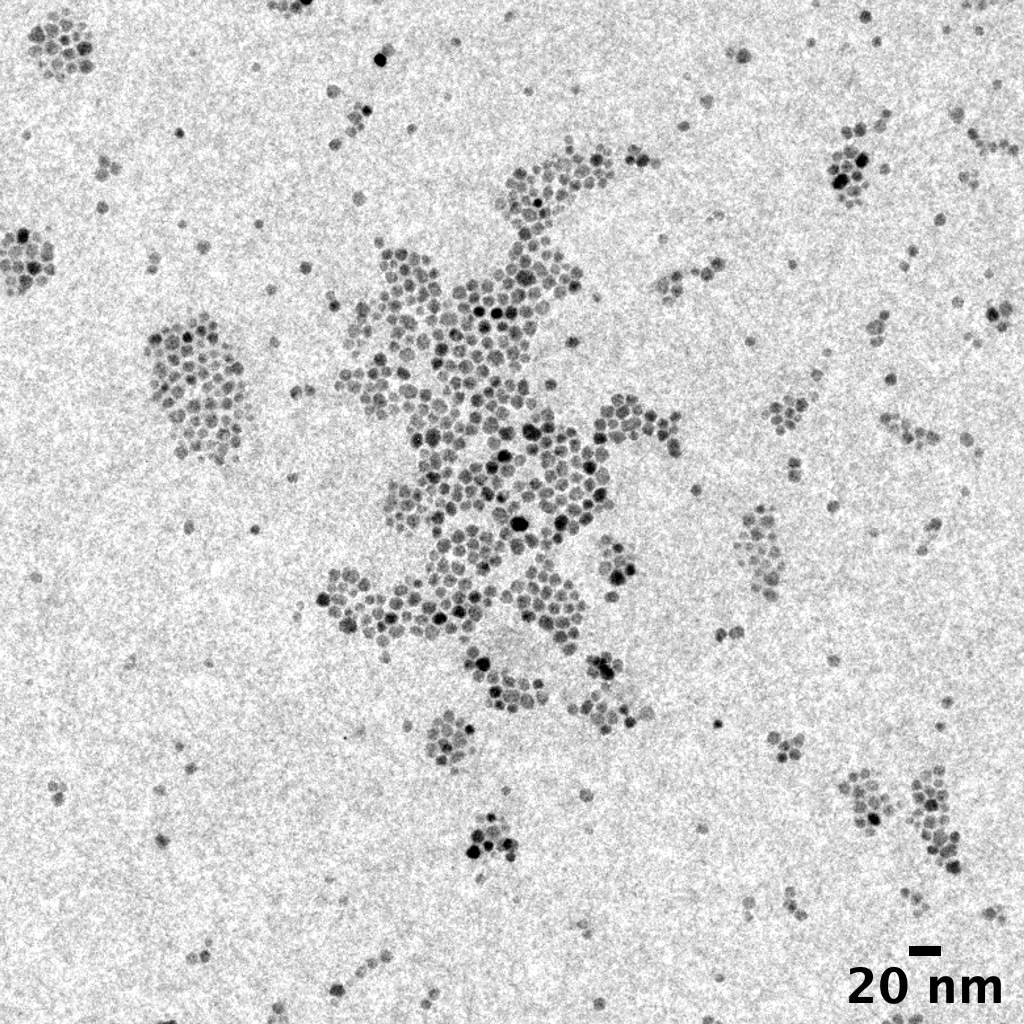
\includegraphics[width=\linewidth]{images/tem5.png}
	\end{subfigure}
	\begin{subfigure}[b]{0.25\textwidth}
		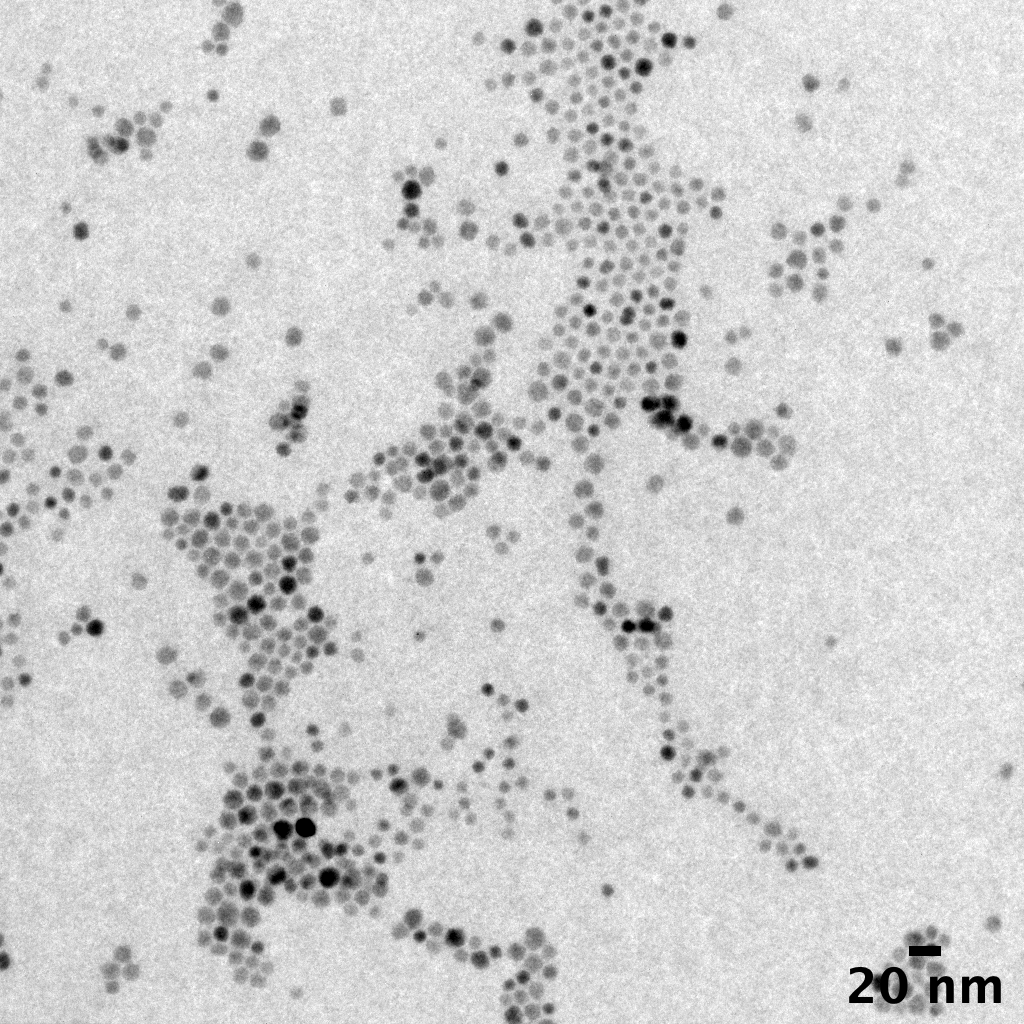
\includegraphics[width=\linewidth]{images/tem10.png}
	\end{subfigure}
	\begin{subfigure}[b]{0.25\textwidth}
		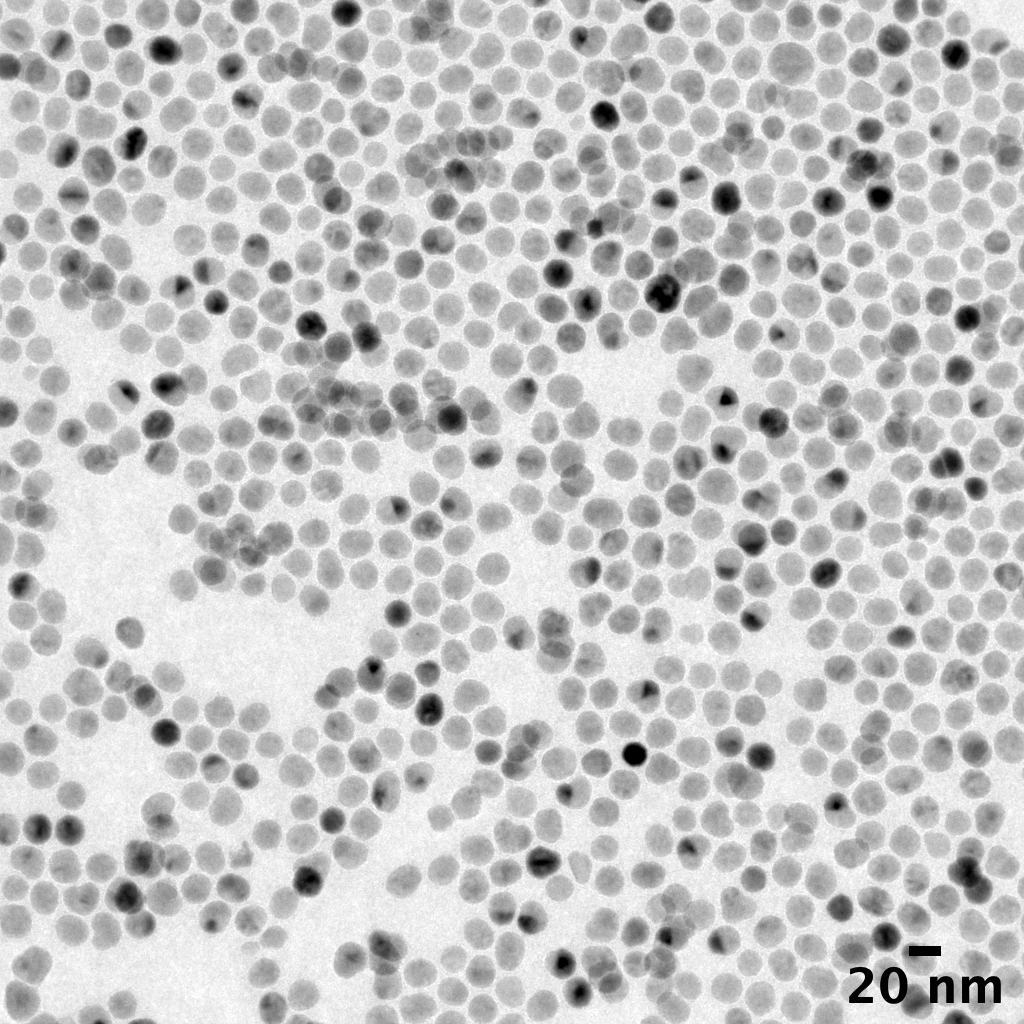
\includegraphics[width=\linewidth]{images/tem20.png}
	\end{subfigure}
\par\smallskip
	\begin{subfigure}[b]{0.25\textwidth}
		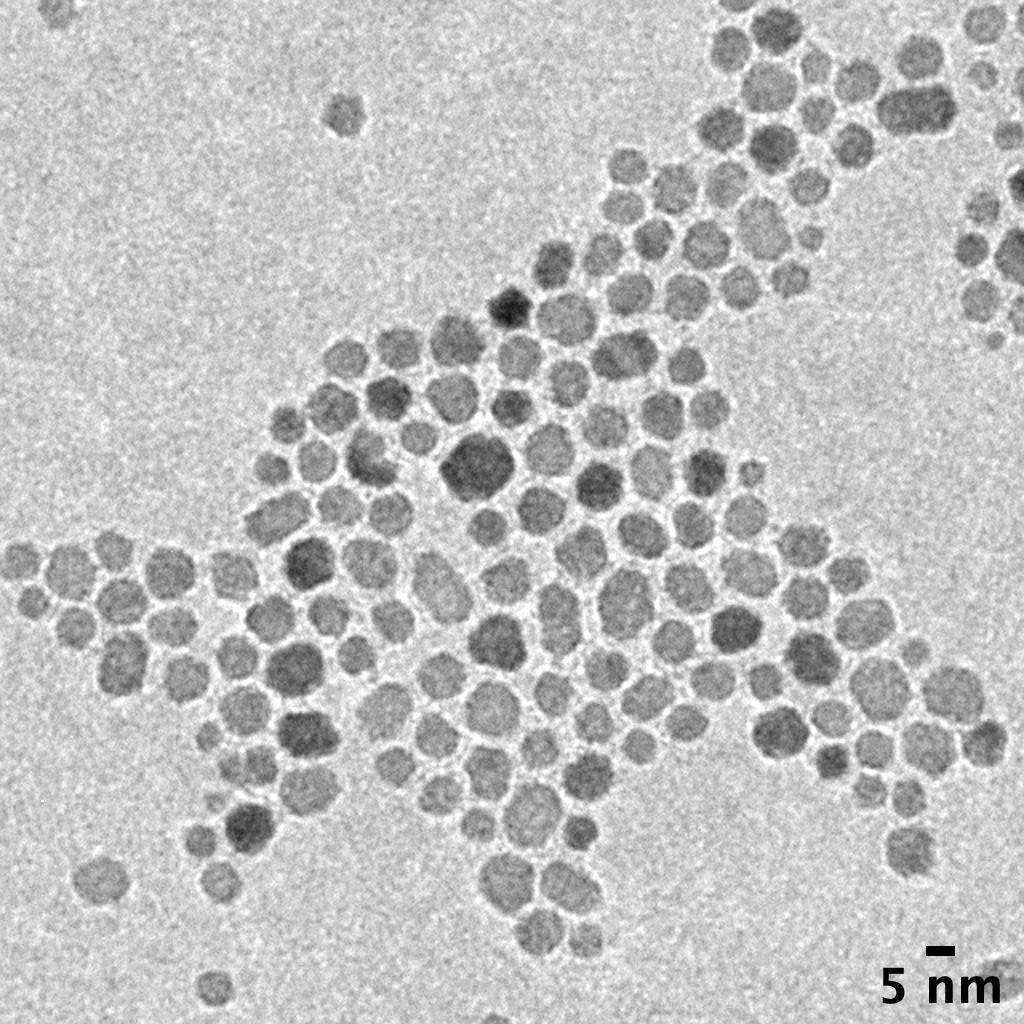
\includegraphics[width=\linewidth]{images/temh5.png}
	\end{subfigure}
	\begin{subfigure}[b]{0.25\textwidth}
		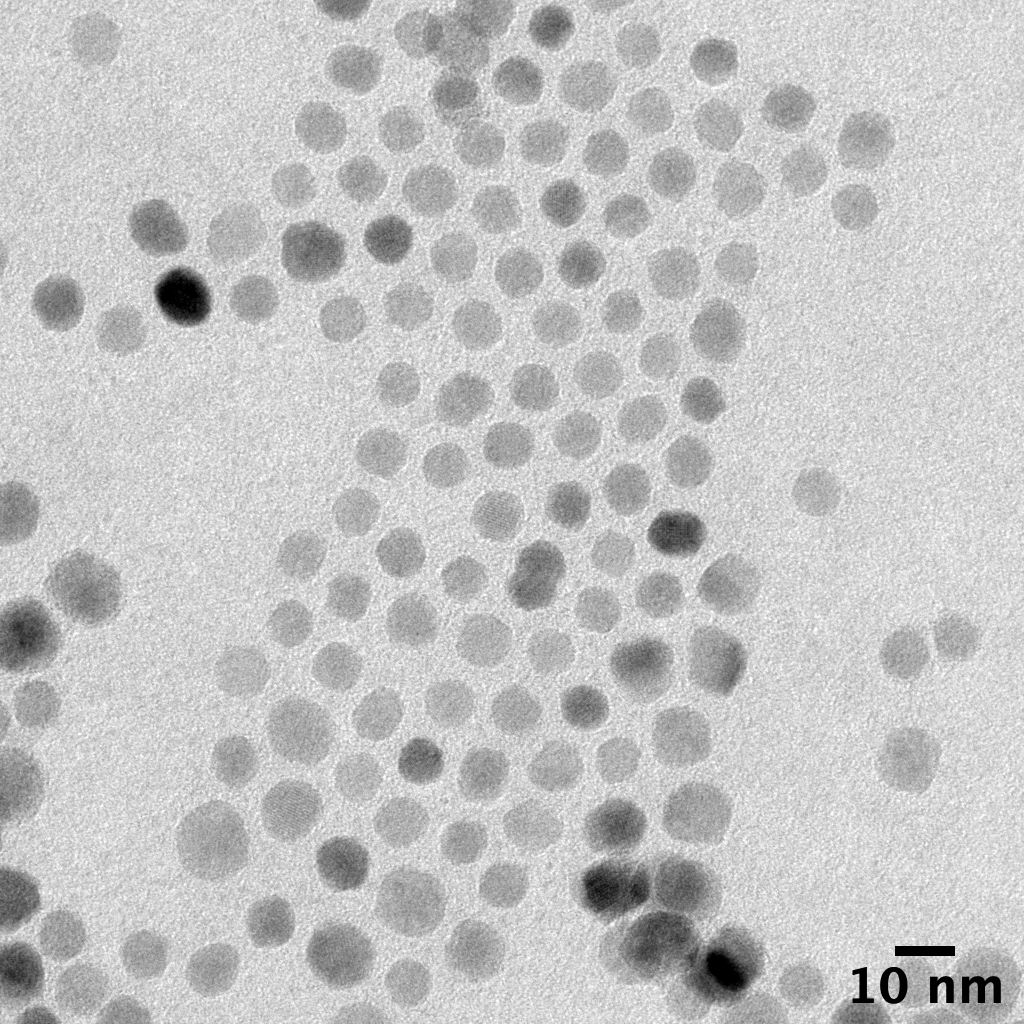
\includegraphics[width=\linewidth]{images/temh10.png}
	\end{subfigure}
	\begin{subfigure}[b]{0.25\textwidth}
		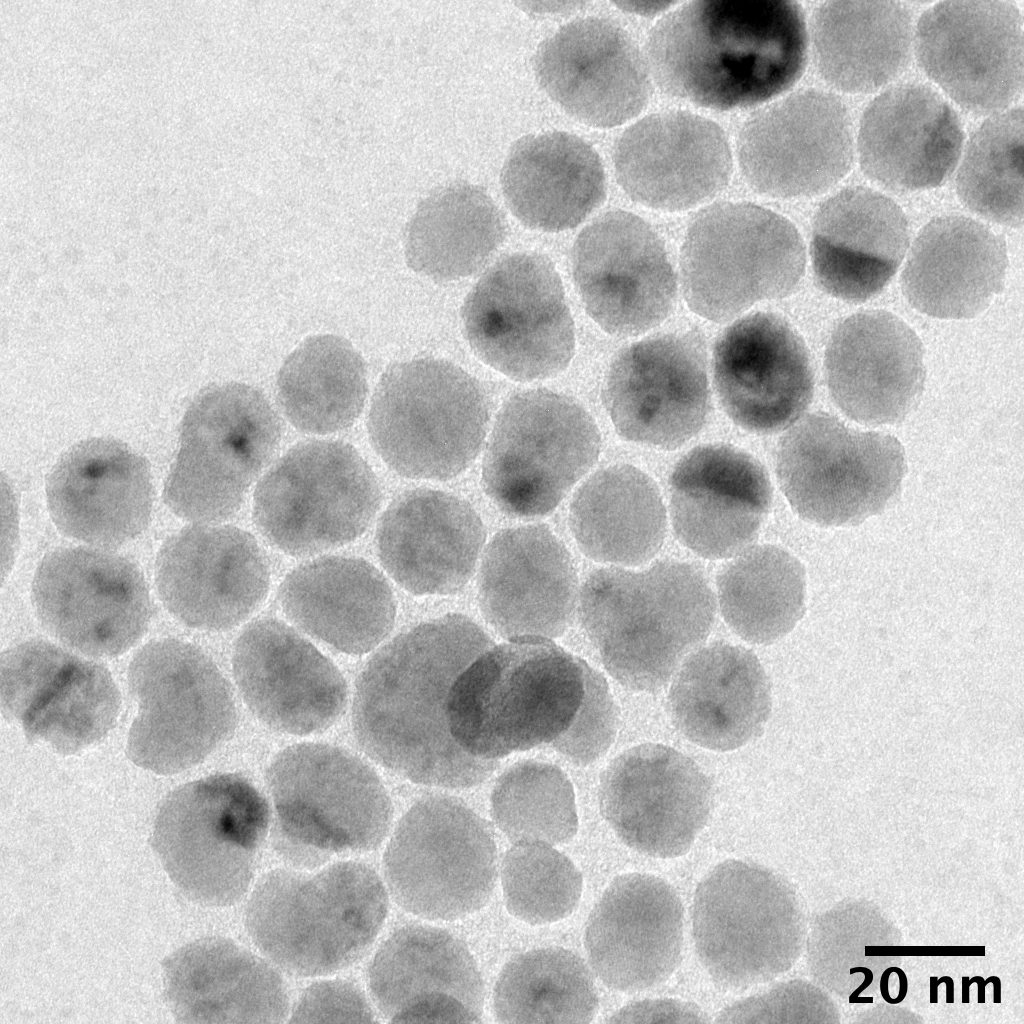
\includegraphics[width=\linewidth]{images/temh20.png}
	\end{subfigure}
\caption[TEM images of iron oxide nanoparticle]{TEM images of the iron oxide nanoparticles. From left to right: 5\,nm 10\,nm and 20\,nm nominal size in two different magnifications each (rows).}
\label{fig:tem}
\end{figure}
.


SAXS measurements of the prepared nanoparticle polymer foils where performed at the SSRL beamline 1-5. Samples were measured at 12\,keV for at two different spots for 5\,min each and averaged, a subtraction of the polymer matrix background was performed and a size distribution of spherical particles with hardsphere interaction was fitted to the radial profile. The low-q area is dominated by aggregate formation, which cannot be precisely quantified due to stray light and limited measuring range and is accounted for by a guinier-porod function, see \fref{fig:saxsps}  and  \fref{fig:saxspmma} \cite{percus1958,feigin1987,Ilavsky2009}.
The measurements do not show a clear and significant difference between the two polymer matrices. According to the regressions, the aggregates seem to have a radius of gyration of 20-30\,nm (the straylight limits the measurement validity in those small q areas), the porod $P$ of 2.5-3.8 suggests a dimensionality of the aggregates between 2 and 3.  \cite{feigin1987,lili2005}. The radii of the form factor agree within the corresponding margin of error with the values of determined by TEM measurements, the difference between the radius parameters of the structure factors and the form factor is most likely caused by the thin layer of oleic acid ligands between aggregating particles.


\begin{figure}[tp]
	\centering
	\begin{subfigure}[b]{0.3\textwidth}
		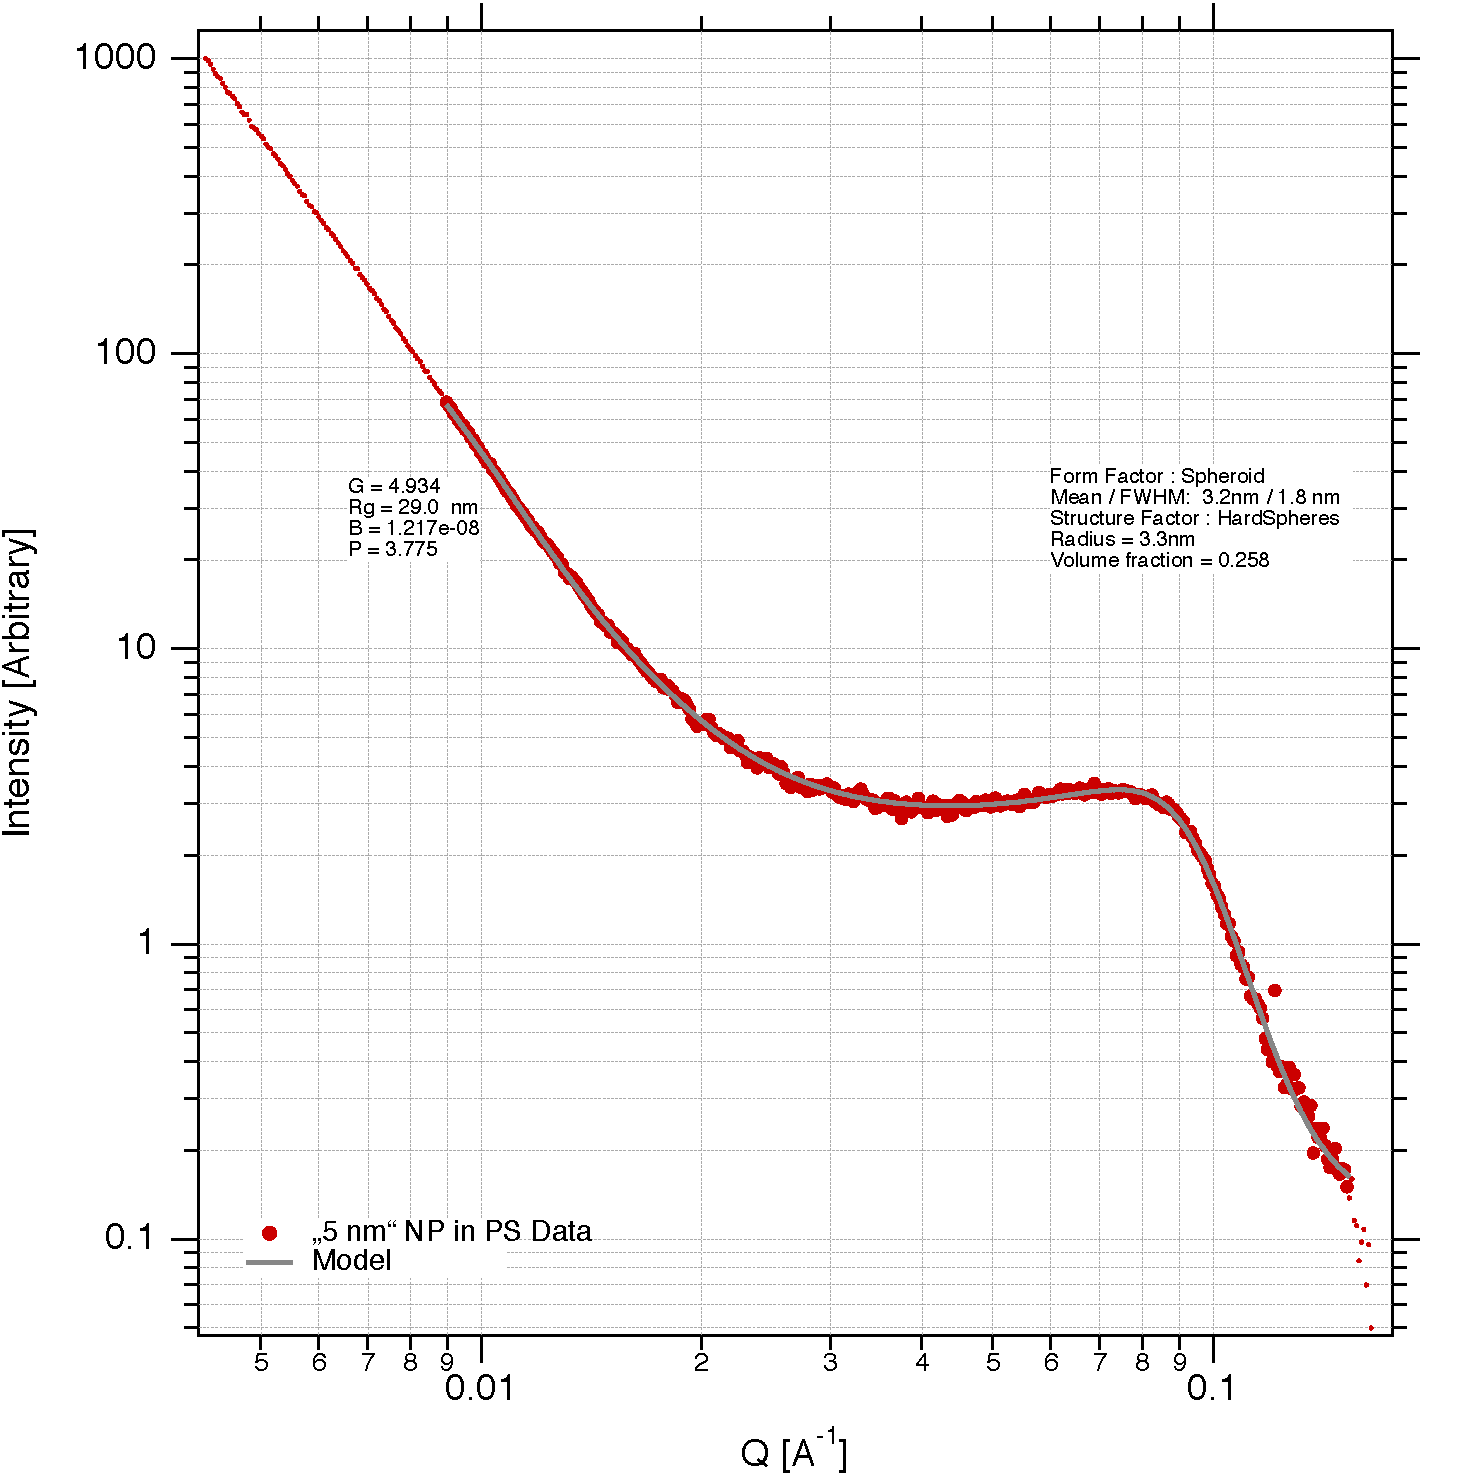
\includegraphics[width=\linewidth]{images/ps5.pdf}
	\end{subfigure}
	\begin{subfigure}[b]{0.3\textwidth}
		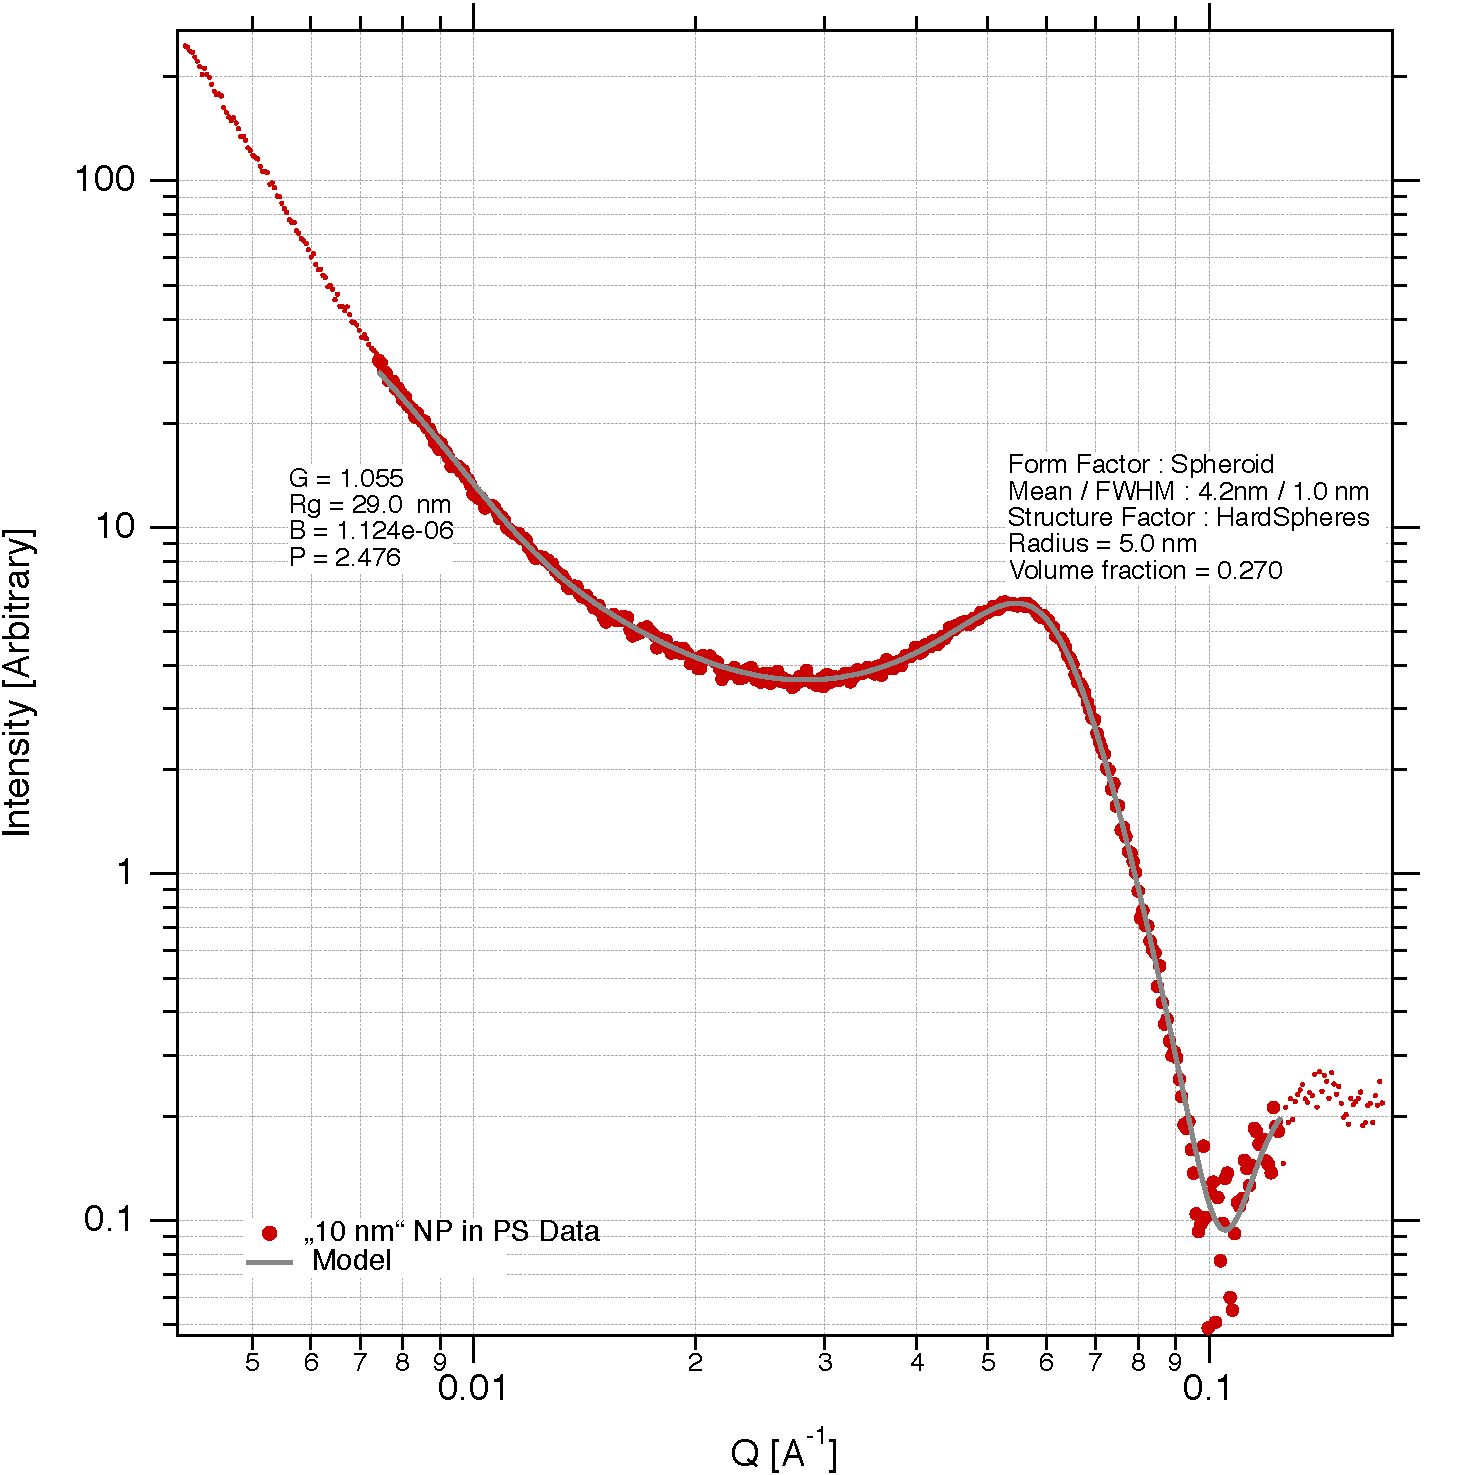
\includegraphics[width=\linewidth]{images/ps10.pdf}
	\end{subfigure}
	\begin{subfigure}[b]{0.3\textwidth}
		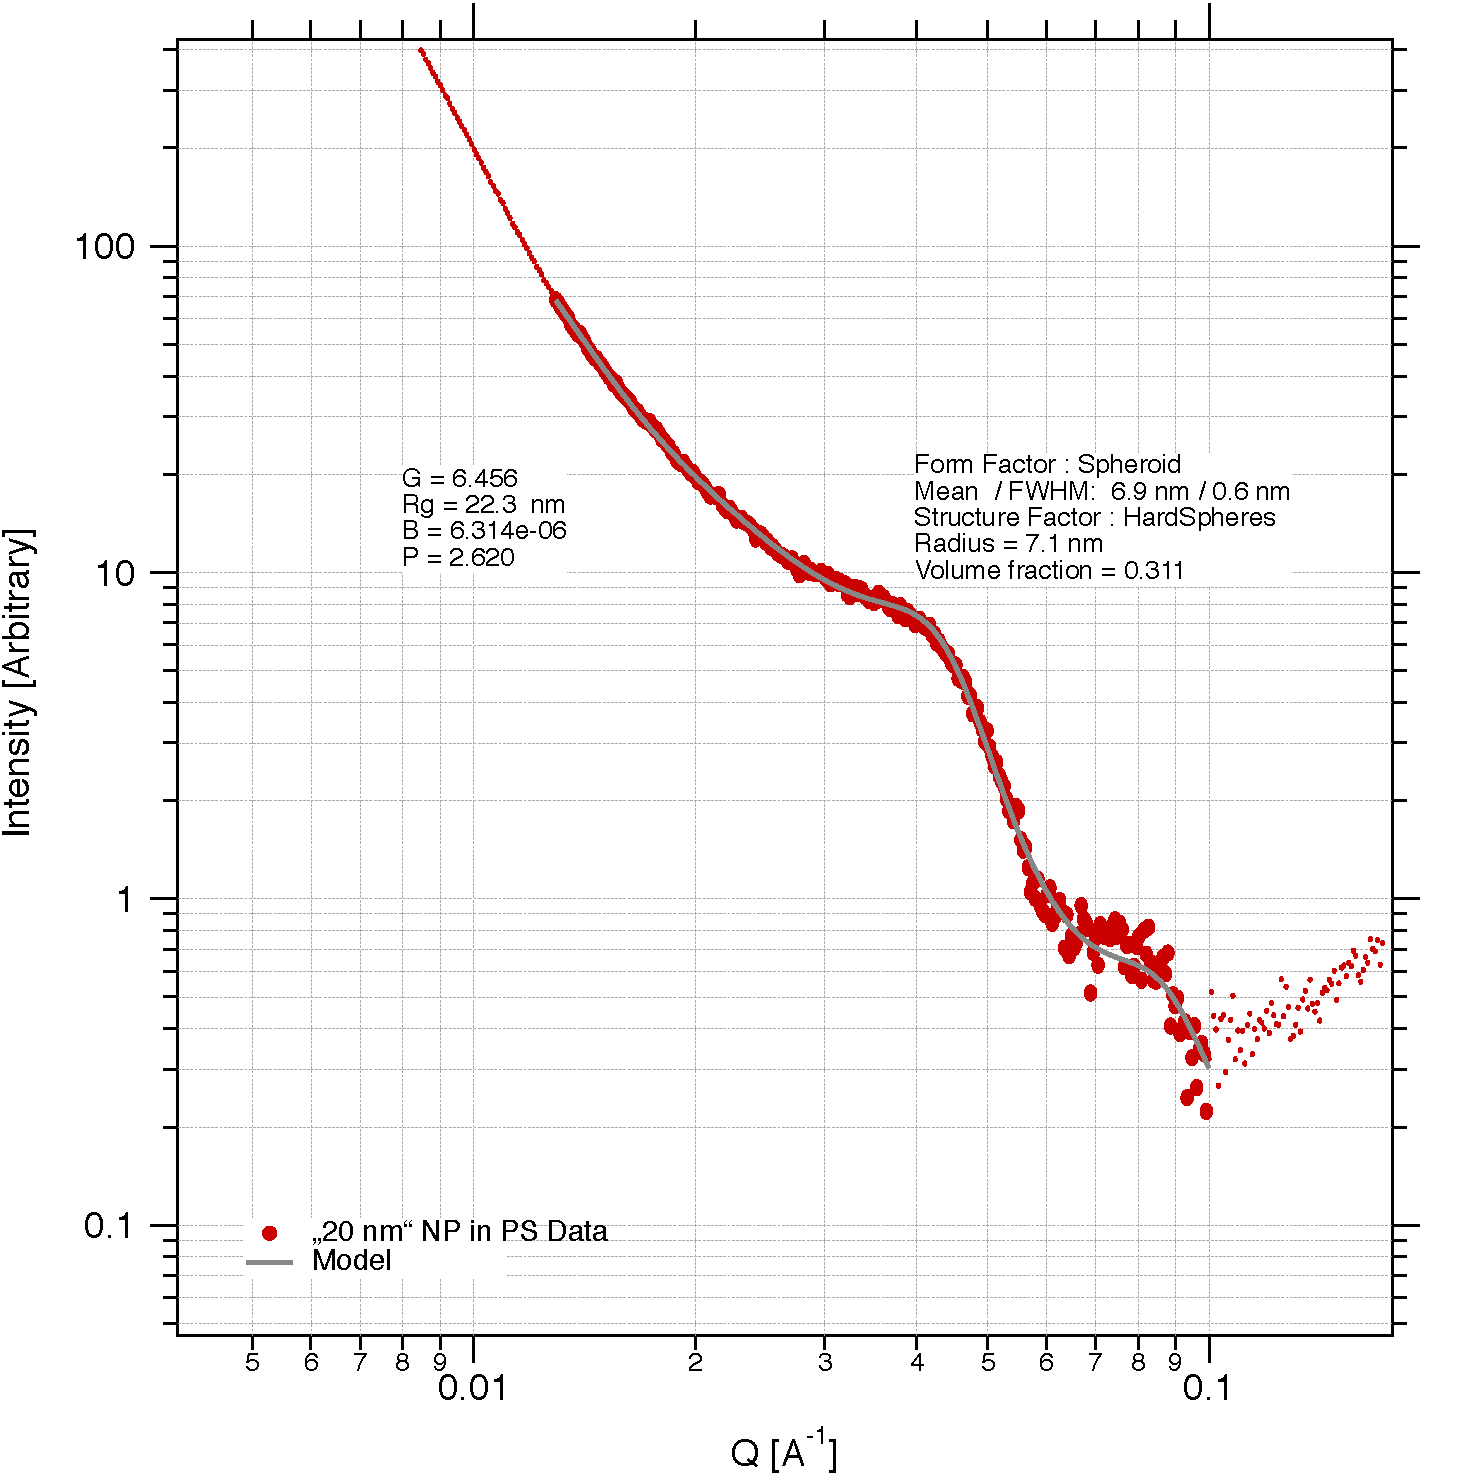
\includegraphics[width=\linewidth]{images/ps20.pdf}
	\end{subfigure}

	\caption[SAXS profile of iron oxide nanoparticles in polystyrene matrix]{SAXS profiles of nominal 5\,nm, 10\,nm and 20\,nm iron oxide nanoparticles in polystyrene matrix (left to right).}
	\label{fig:saxsps}
\end{figure}
\begin{figure}[tp]
	\centering
	\begin{subfigure}[b]{0.3\textwidth}
		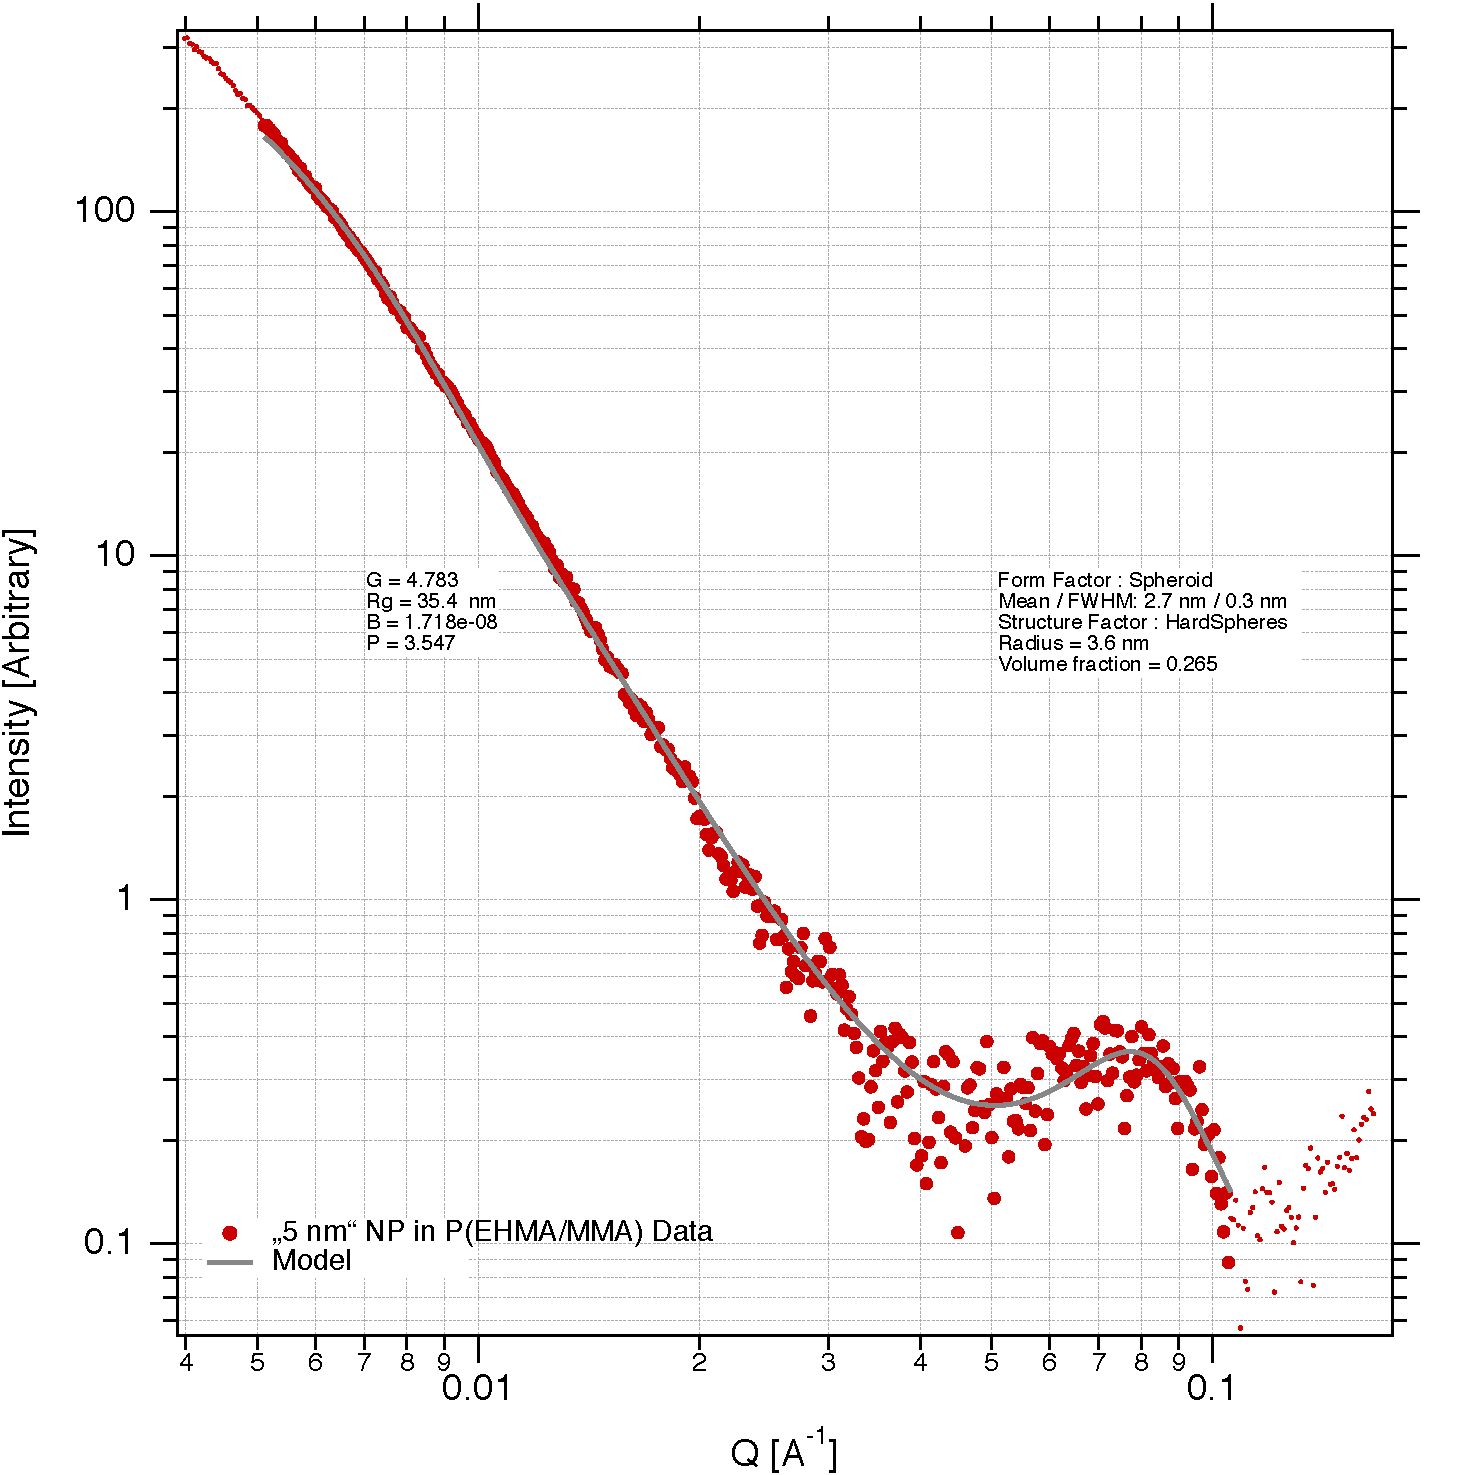
\includegraphics[width=\linewidth]{images/pmma5.pdf}
	\end{subfigure}
	\begin{subfigure}[b]{0.3\textwidth}
		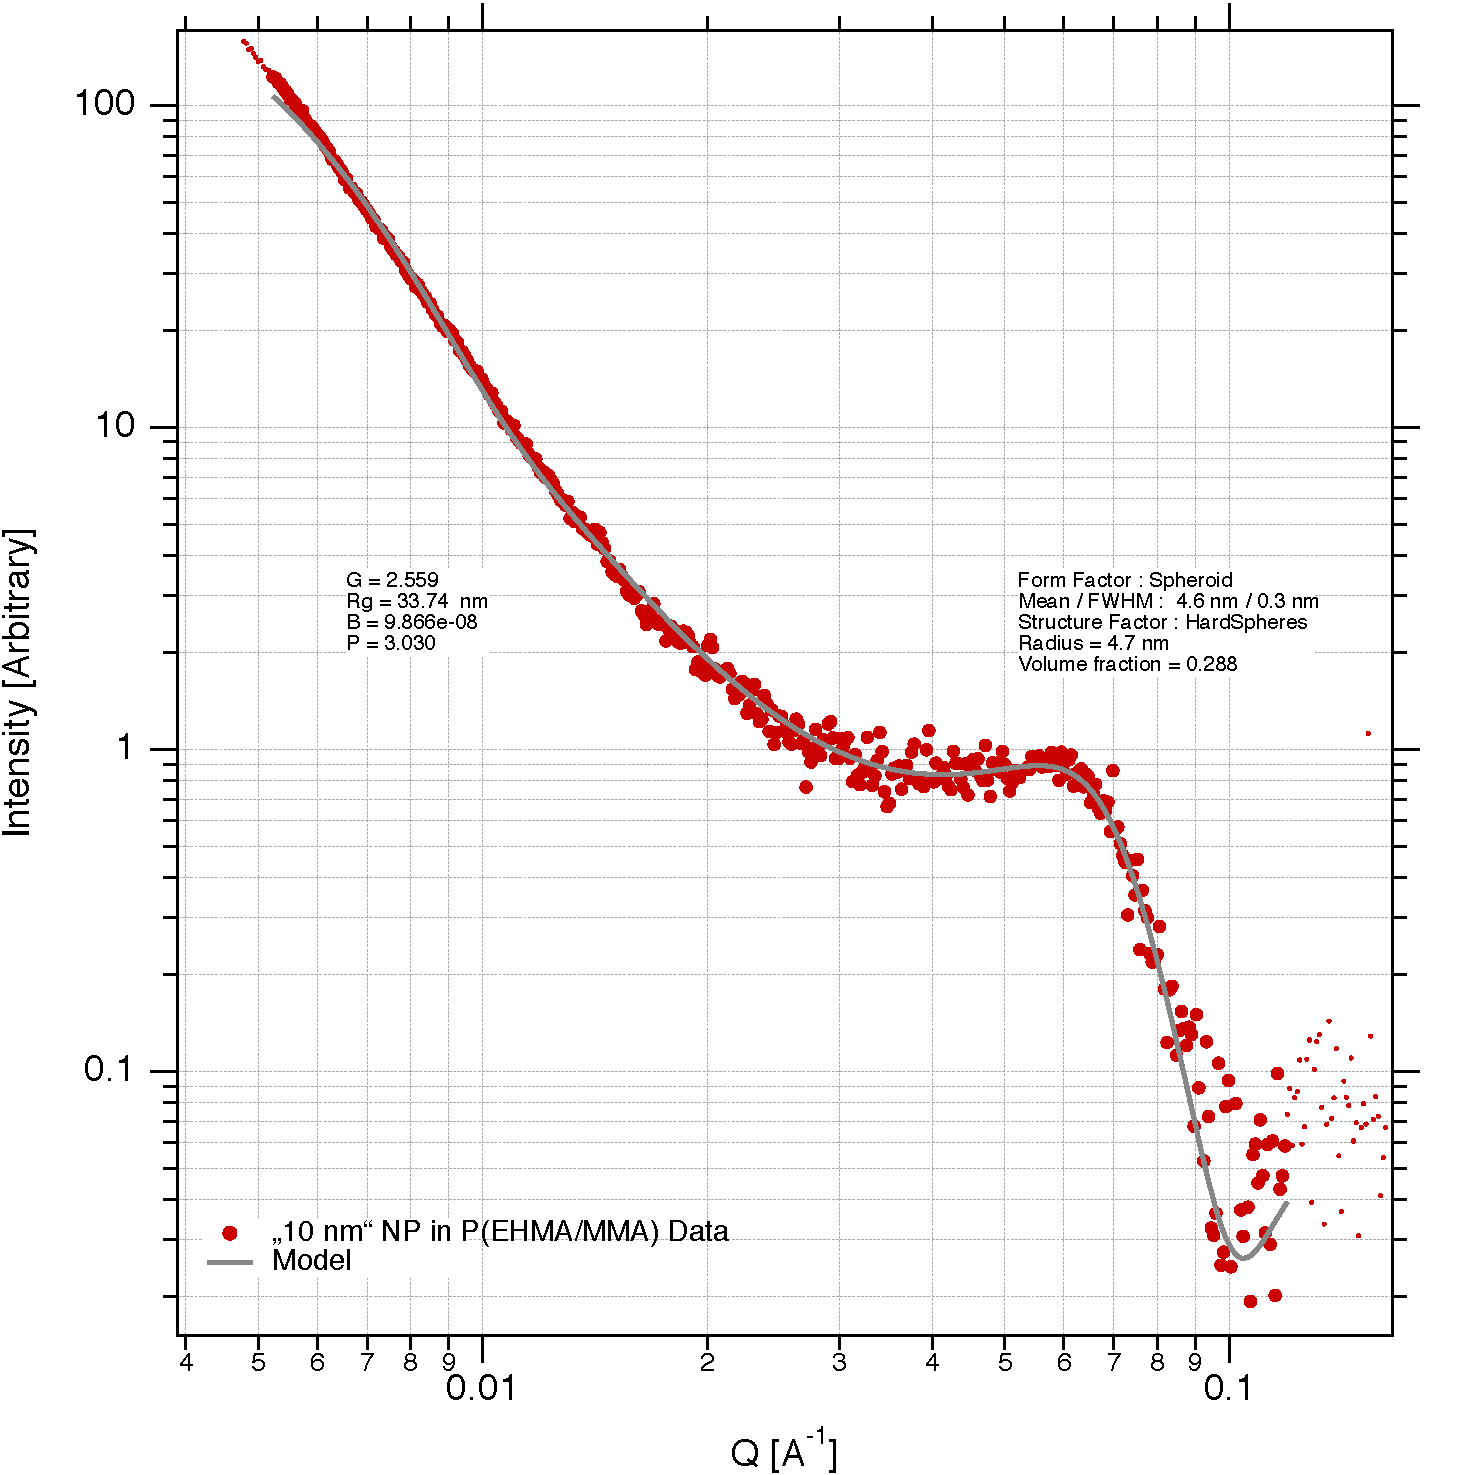
\includegraphics[width=\linewidth]{images/pmma10.pdf}
	\end{subfigure}
	\begin{subfigure}[b]{0.3\textwidth}
		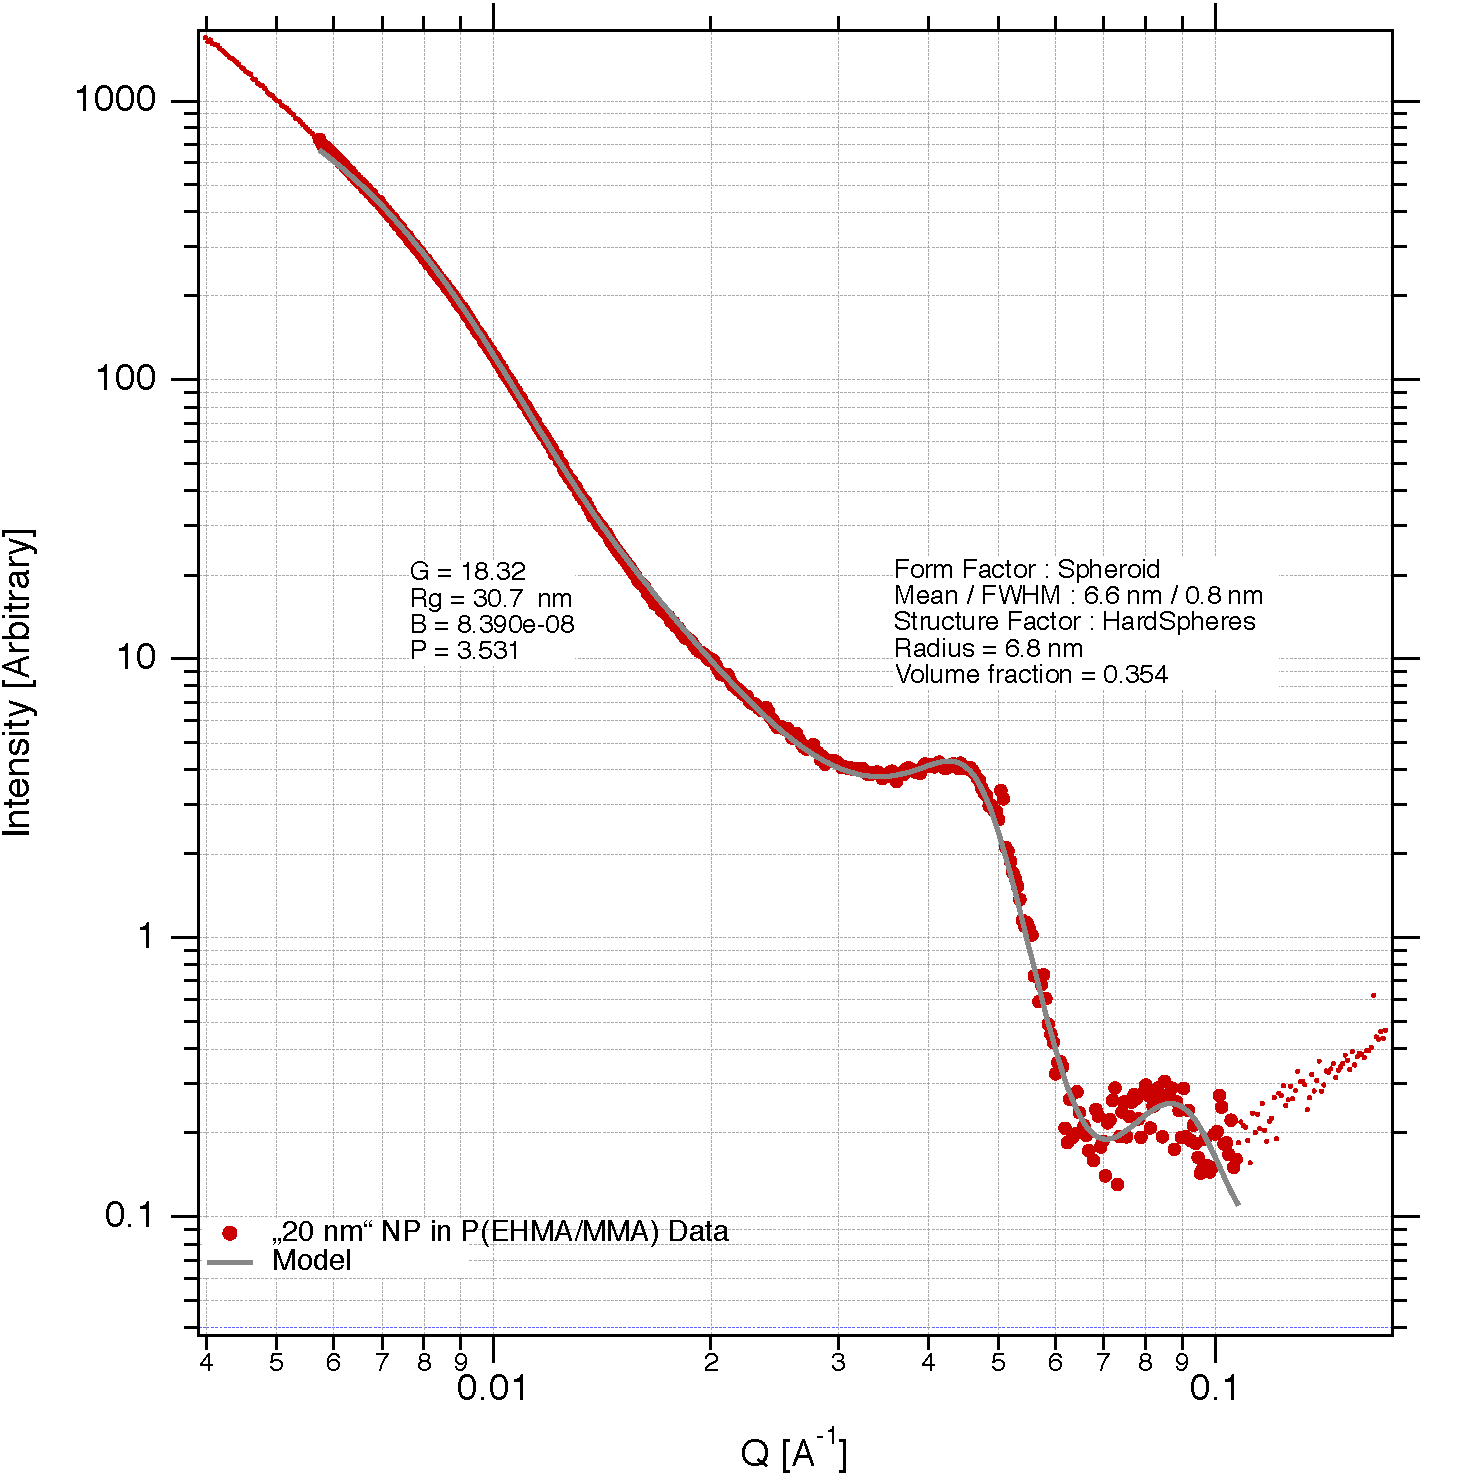
\includegraphics[width=\linewidth]{images/pmma20.pdf}
	\end{subfigure}
	
	\caption[SAXS profile of iron oxide nanoparticles in  Poly-(EHMA/MMA) matrix]{SAXS profiles of nominal 5\,nm, 10\,nm and 20\,nm iron oxide nanoparticles in Poly-(EHMA/MMA) matrix (left to right).}
	\label{fig:saxspmma}
\end{figure}

The SAXS measurements give a reasonably good insight into the expected results of the IDI scheme measurement of the same sample, which will differ due to the iron specificity and the smaller focal volume in the latter.  

\subsection{GaAs Crystal Films}
As a crystalline sample GaAs was chosen for its simple fcc structure and large product of the gallium K-shell fluorescence Energy and lattice constant. The samples were prepared by Ben Reeves at the Stanford Nanofabrication Facility. 
Using MOCVD, 50\,nm GaAs, 400\,nm AlGaAs as an etch stop and finally a 5\,um GaAs film were grown on an epi-ready (100)±0.1° GaAs substrate. The speciman was cut into 12\,mm\,x\,15\,mm pieces, each glued to an approx. 100\,um thick fused silica cover slip with the 5\,um film layer facing towards the silica. The substrate and the AlGaAs layer were selectively etched away via C6H8O7:H2O2 and HF:H2O wet etches, respectively. This left 5\,um thin GaAs films glued onto the the quartz slides (see \fref{fig:gaas_sample}).  XRD with Cu K-alpha was used to measure the width of the (004) GaAs bragg peak as 0.004°, indicative of high quality single crystals. 

\begin{figure}[tp]
	\centering
	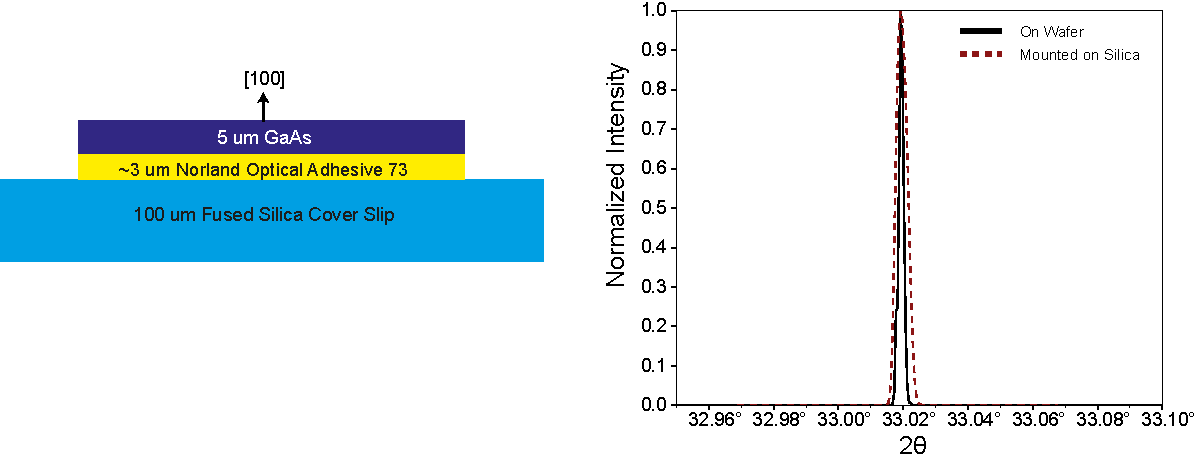
\includegraphics[width=0.8\linewidth]{images/gaas_sample.pdf}
	\caption[GaAs Sample]{Sketch of the GaAs single crystal glued to a fused silica cover slip and Cu-K$\alpha$ XRD measurement of the GaAs (004) reflex, showing a single crystal. After mounting on the cover slip, the peak is slightly broadened, most likely by an slighly uneven thickness of the glue layer. }
	\label{fig:gaas_sample}
\end{figure}


\section{Setup}
The setup used at EH5 at SACLA is shown in \fref{fig:setup}. 

The sample was mounted in an XXX angle to the beam on an XXX axis stage to allow scanning of the sample, ensure perpendicularly of the scanning directions to the beam to stay within the Rayleigh length of approx. XXX\,um while also ensuring a parallel alignment of the sample surface to one of the detectors. Overall, two MPCCD detectors were used: A Dual detector with two tiles, each 512x1024 pixels perpendicular to the FEL beam in a distance of 1\,m and a Short Working Distance Octal detector, consisting of eight 512x1024 tiles, parallel to the sample surface in a distance $d_{octal}$ ranging from XXX to XXX cm. To supress absorption and more importantly, air scattering, a vacuum pipe with Kapton windows was installed in between the sample and the Dual detector
An L-shaped aluminum plate was installed to reduce stray light as well as to allow mounting of the beamstop and filters to suppress coherent scattering and K$\beta$ fluorescence and between sample and detector.
\begin{figure}
	\centering
	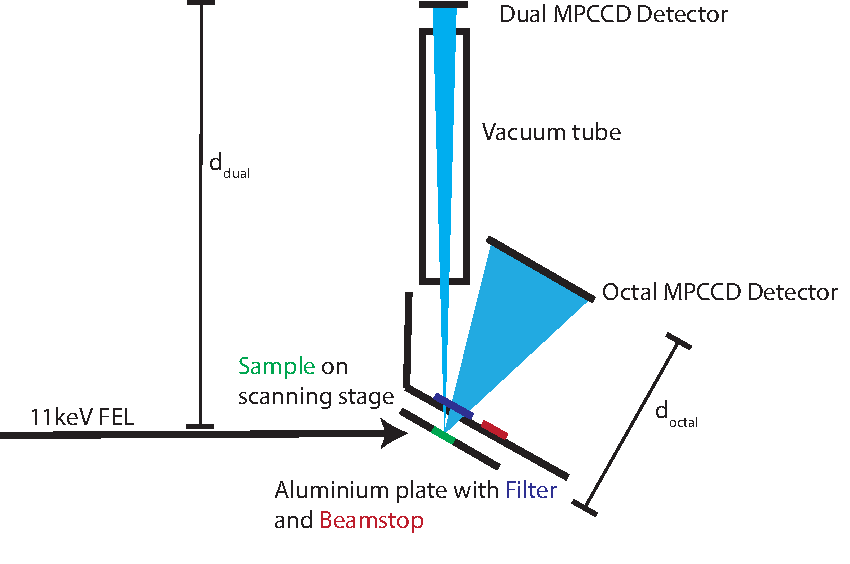
\includegraphics[width=0.8\linewidth]{images/setup.pdf}
	\caption[Experimental setup at SACLA]{Experimental setup at SACLA: The sample is mounted on a scanning stage and aligned to stay in focus during the scan and be parallel to the Octal MPCCD detector, which is in a distance $d_{octal}$. The angle between incoming FEL and Sample is XXX. Behind the sample, a stray light filter, beamstop and (depending on the sample) a filter foil is installed. The Dual detector is mounted $d_{dual}$=1\,m away from the sample in a XXX angle. To reduce air scattering, a vacuum tube is installed in the path from sample to Dual.}
	\label{fig:setup}
\end{figure}
\paragraph{Imaging the Focus}
The image to focus, 
\paragraph{Imaging Nanoparticles}
\paragraph{Imaging Crystals}

\section{Data Processing}
As the amount of recorded data is huge, an efficient strategy for filtering on shots, preprocessing the data to eliminate interference and finally reconstruction has to be implemented.
\subsection{Preprocessing}









\begin{figure}
	\centering
	\begin{subfigure}{0.2\textwidth}
		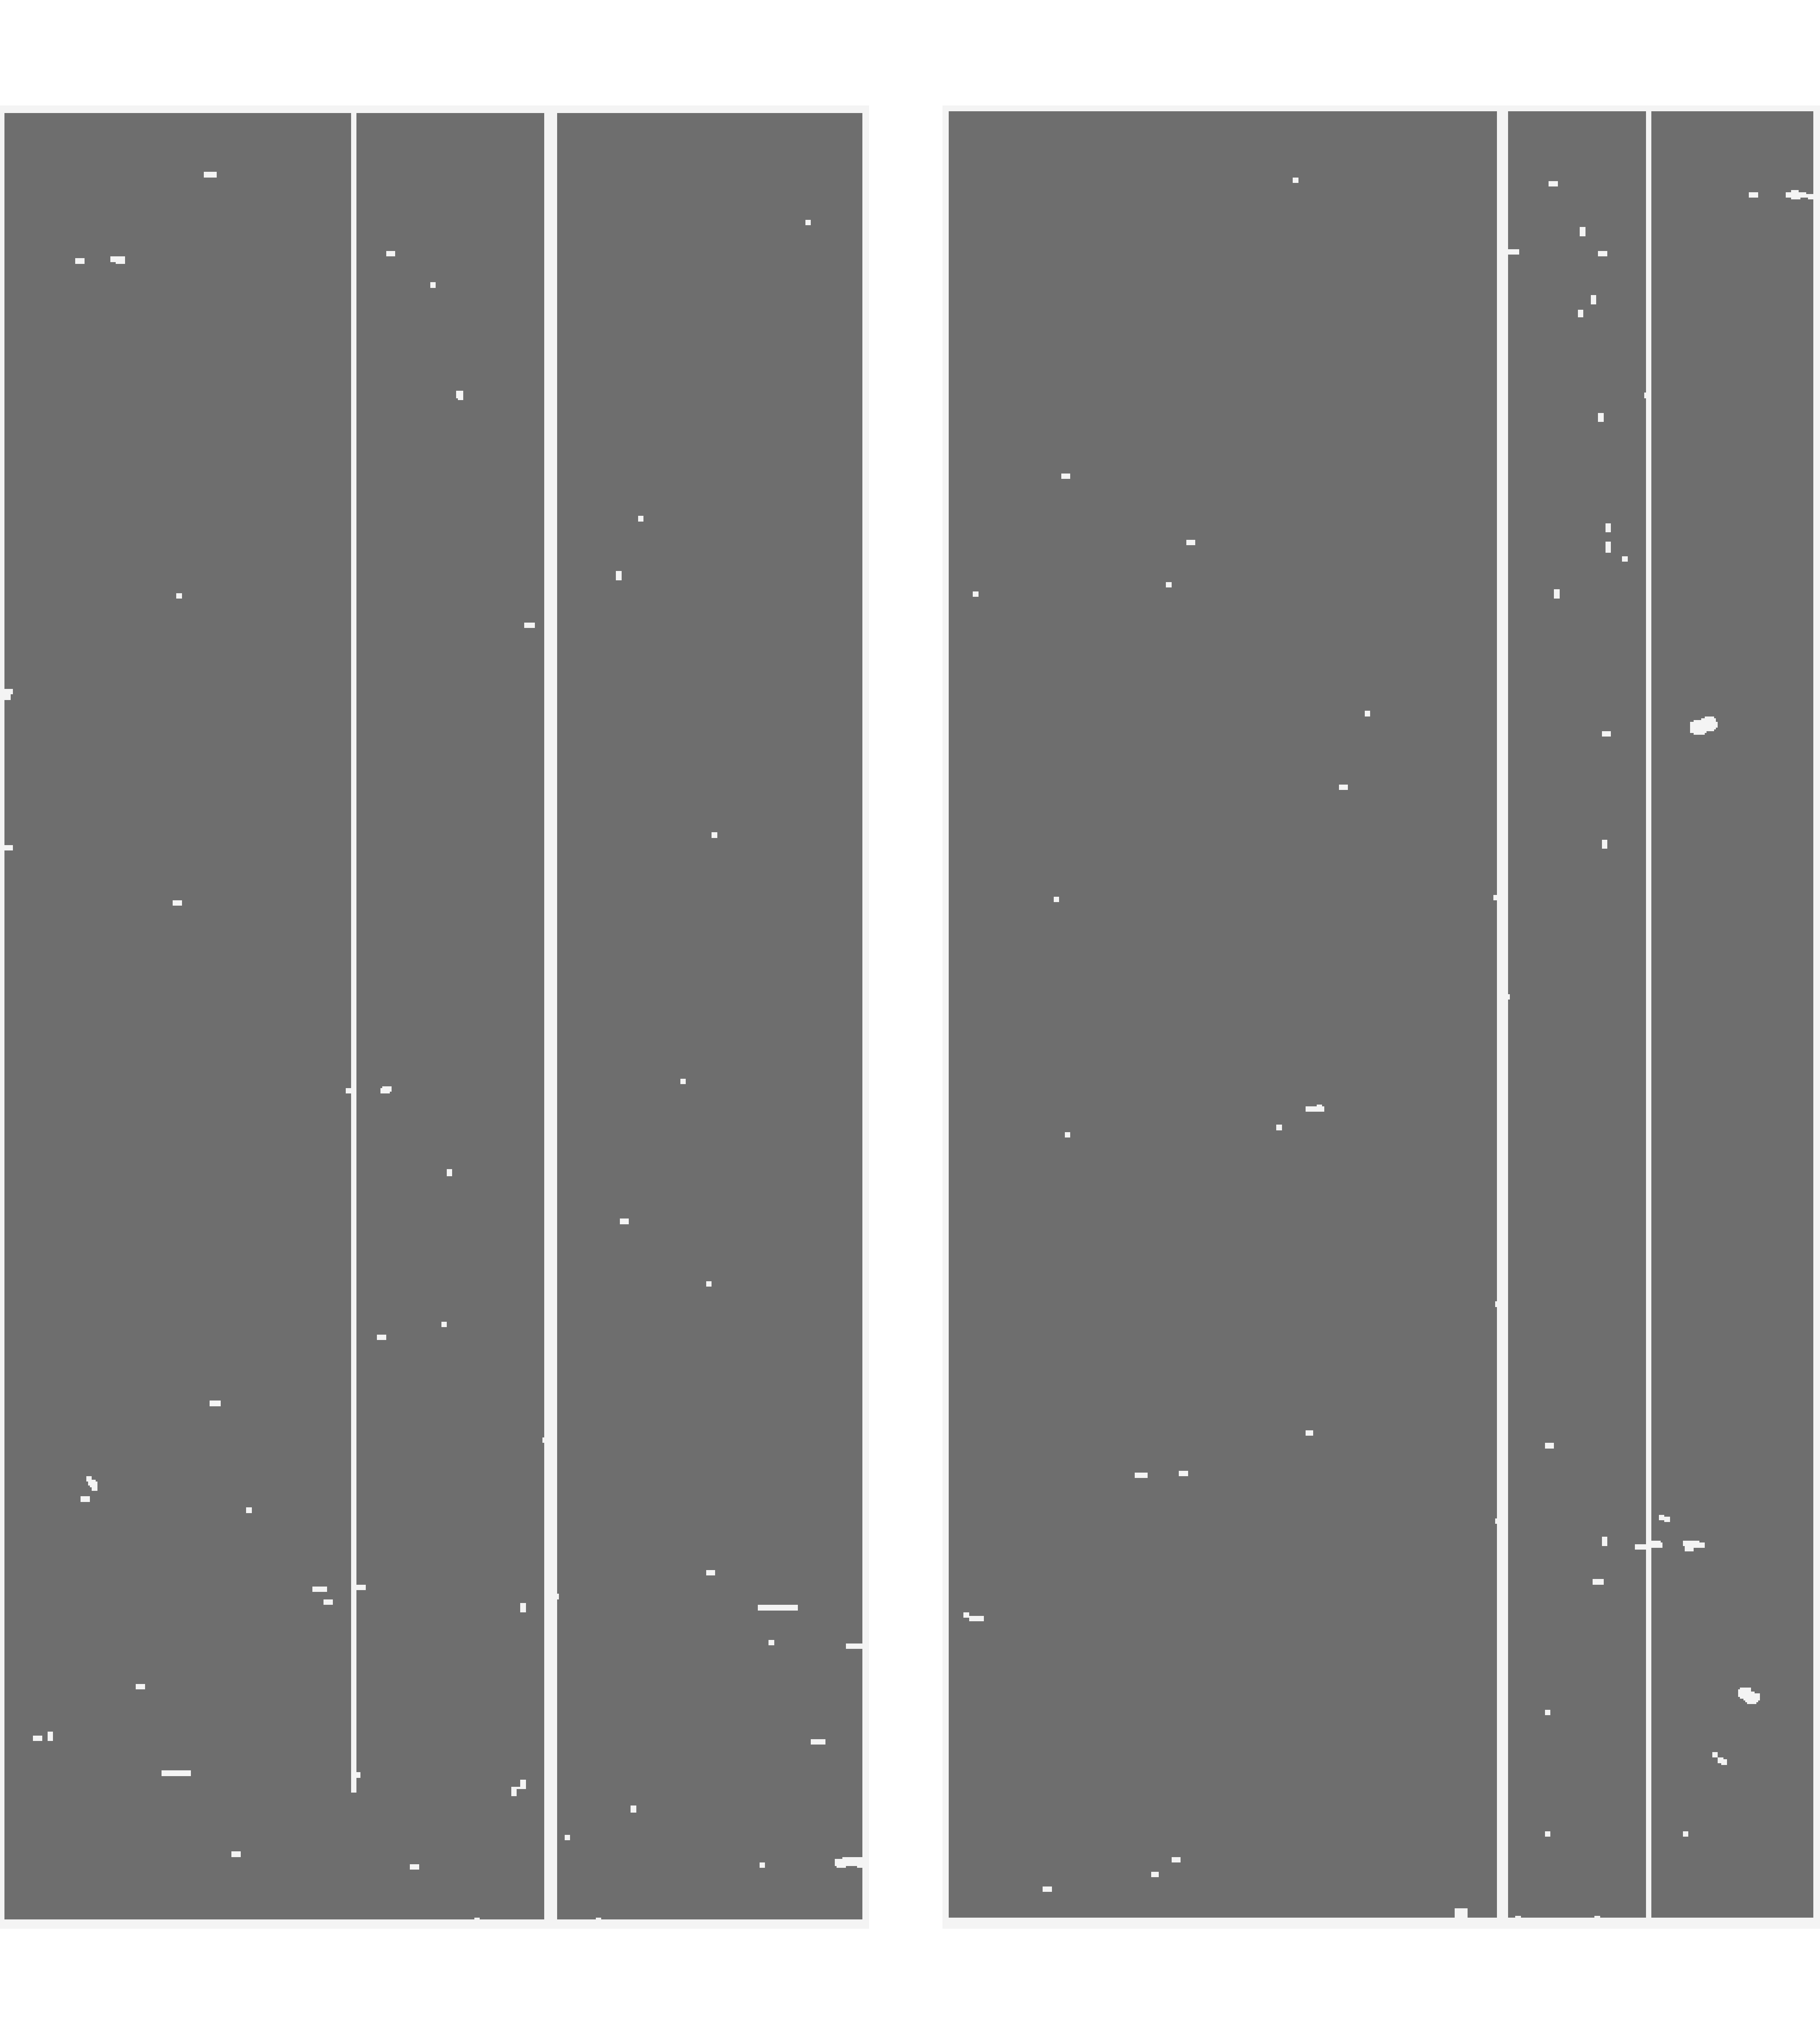
\includegraphics[width=\linewidth]{images/mask_dual.png}
	\end{subfigure}
	\hspace{1cm}
	\begin{subfigure}{0.2\textwidth}
		
\includegraphics[width=\linewidth]{images/mask_octal.png}
	\end{subfigure}
	\caption[Usable detector area]{Usable detector area (gray) of the dual (left) and octal (right) detector after signal correction and statistical filtering. Only the intersection of good areas for each run will be used. This way the same mask and number of correlation pairs will be used for samples that will be compared to each other.}	
\end{figure}

\paragraph{Shot filtering}
A first rough filtering pass on the recorded data is done on the following criteria: Reported beam energy > XXX, beam energy in the hutch being not more than one standard deviation below the mean energy and the distance on the sample to the closest neighboring shot not being less than one standard deviation of the mean distance to the next neighbor for the sample (to remove shots with stopped, turning or still accelerating scanning motors). Furthermore, the scanning range occupied by the sample is identified by the fluorescence intensity on the octal detector and shots, were the X-ray beam does not hit the sample are removed.

\paragraph{Filtering for Impurities}
On some of the samples, areas can be identified where the relative fluorescence intensities at different energies change. An example is shown in \fref{fig:xrf}: For a 500\,nm thick iron foil, a spot can be seen where the intensity at 8\,keV is much higher than expected. As this is most likely due to impurities on the sample, those areas are identified and excluded from further analysis.

\begin{figure}
	\centering
	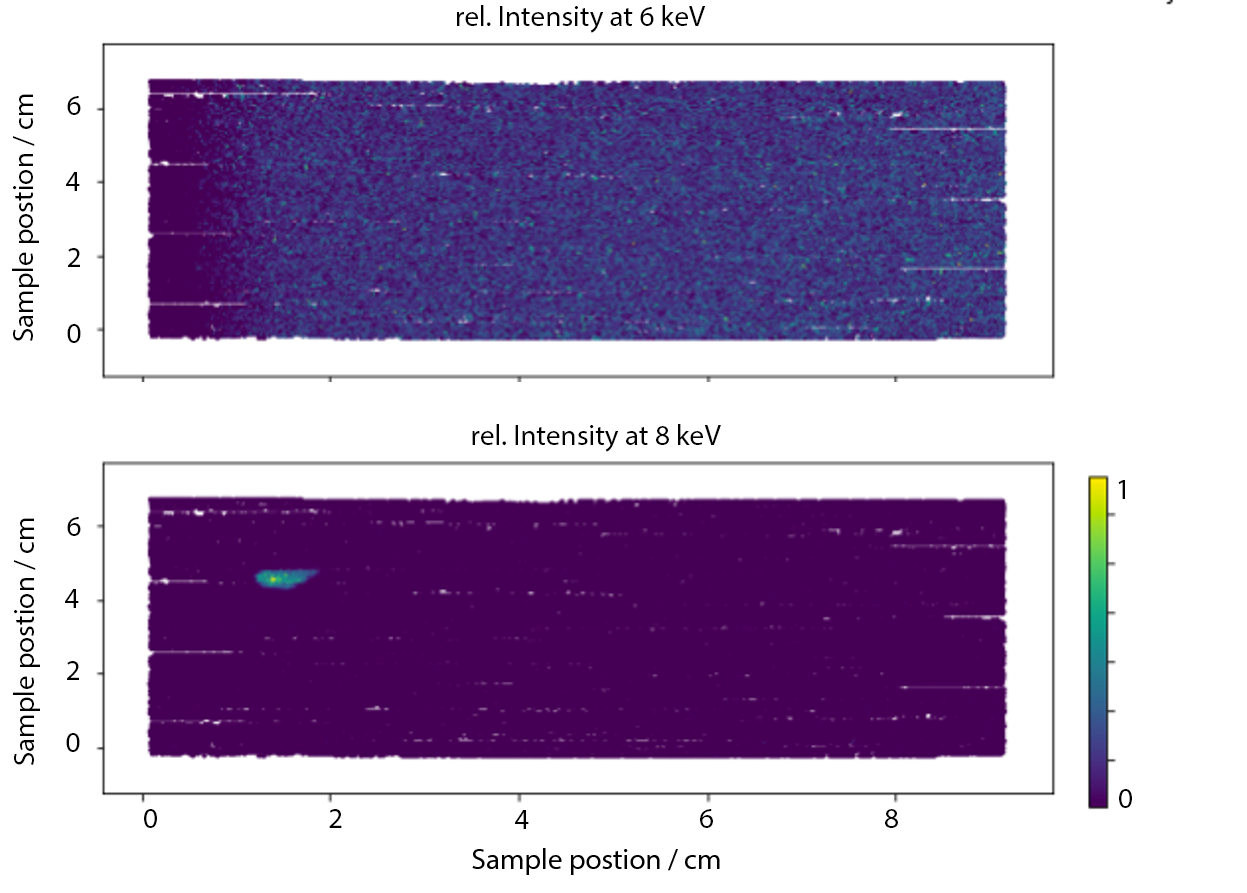
\includegraphics[width=0.7\linewidth]{images/xrf.png}
	\caption[Exemplary relative intensity of the 6 keV and 8 keV photon peak on the detector for different scanning positions on the sample]{Exemplary relative intensity of the 6 keV and 8 keV photon peak on the detector for different scanning positions on the sample. In this iron sample, a localized impurity, most likely copper, is clearly visible and can be masked out .}
	\label{fig:xrf}
\end{figure}

\paragraph{Detector masking}

\paragraph{Detector Artifacts}
During the experiment, an unnoticed failure of the electronics of the octal detector has occurred, manifesting as periodic noise on most of the detector tiles at a much higher level than expected (see \fref{fig:octalissue} for an illustration). Not all columns of a tile are affected (in contrast to common-mode effects commonly encountered with different detectors). As the overall affected area of the detector is substantial and the noise leaks through the photon counting scheme by slightly influencing the probability of a pixel being considered a photon hit, causing correlations and therefore artifacts in the reconstruction in one direction, a correction was applied to the affected columns of affected tiles of the detector. For the correction, the median over the affected columns is calculated (for each of the eight separate read out areas of a tile independently) and subtracted. This reduces the artifact, but doesn't fully remove it. As the artifact in the reconstructions is limited to low $q$ compared to the expected positions of the Bragg peaks, no further correction as been applied.

\begin{figure}[tp]
	\centering
	\begin{subfigure}[b]{0.45\textwidth}
		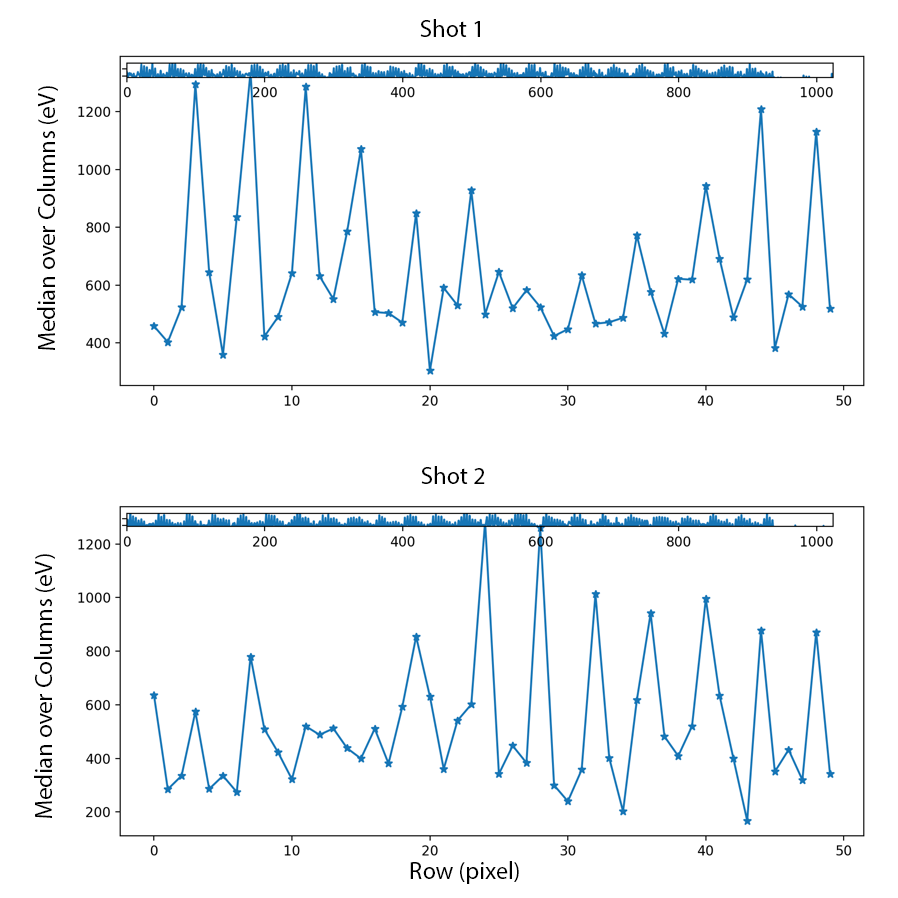
\includegraphics[width=\linewidth]{images/octalissue2.png}
	\end{subfigure}
	\begin{subfigure}[b]{0.45\textwidth}
		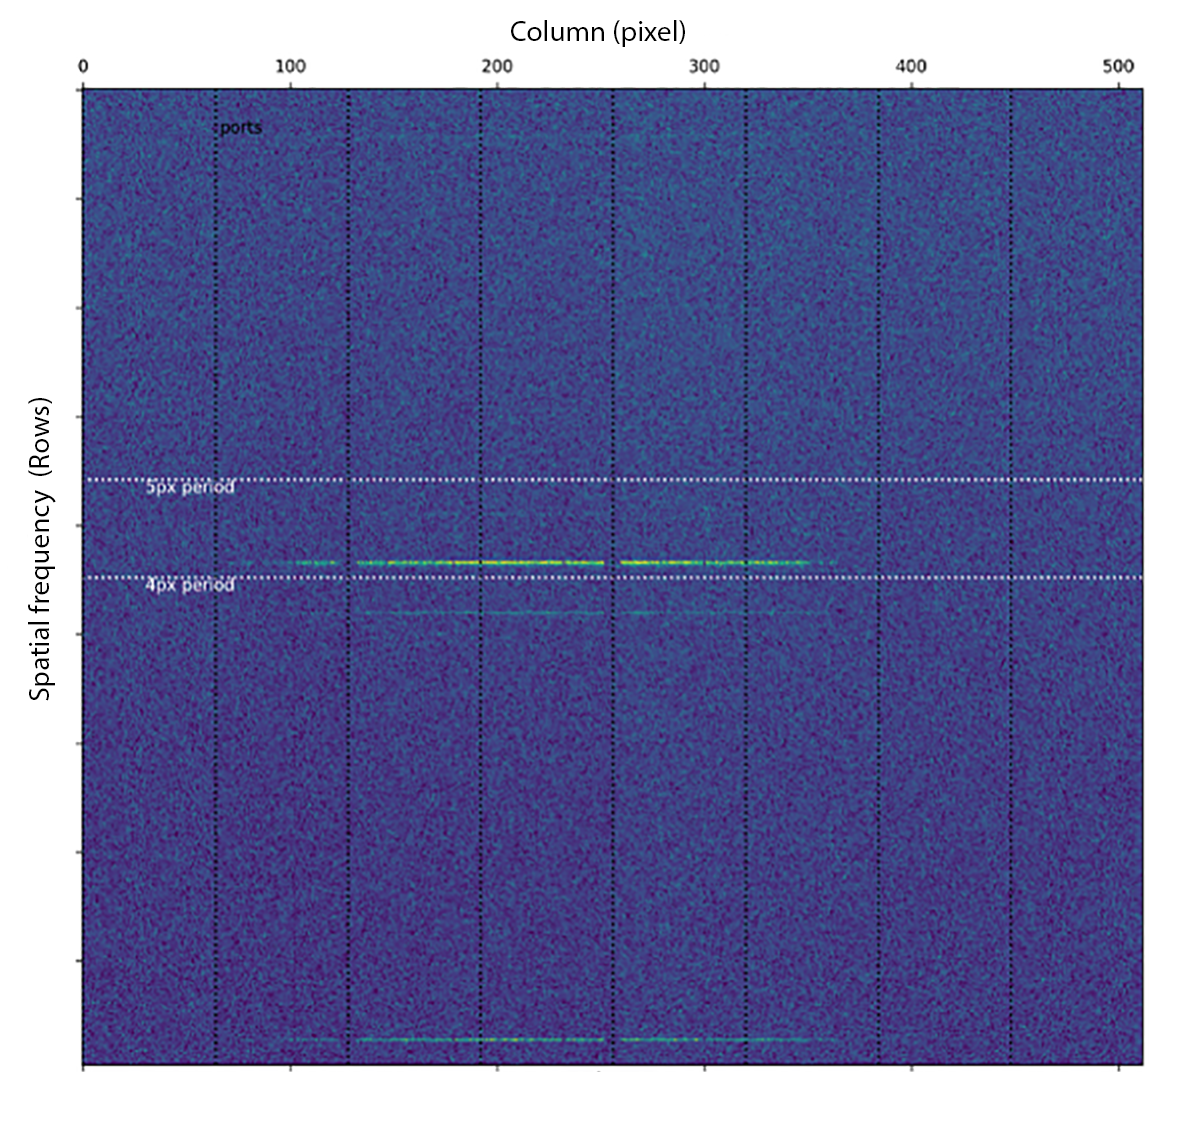
\includegraphics[width=\linewidth]{images/octalissue.png}
	\end{subfigure}
	
	\caption[Periodic noise on octal detector]{Periodic noise on octal detector after background subtraction: For two exemplary shots the median over columns of one detector tile is shown. A periodic noise is visible. The mean spatial spectrum (over the rows) for each column of the tile is shown on the right. The periodic noise is not uniformly affecting all the columns of the tile.}
	\label{fig:octalissue}
\end{figure}


\paragraph{Spectra}
The background subtracted and masked detector images are used to create spectra. On these spectra, a regression with a model consisting of peaks at multiples of the K$_\alpha$ energy and of the excitation energy with an initial FWHM of 500\,eV and intensities following a negative binomial distribution (signal) or Poisson distribution (scattering noise) is performed, minimizing the squared difference the logarithmic values. To roughly approximate the charge sharing, a numerical convolution with a  window of the shape
\begin{equation}
	w (x)= (1-p)\delta(x)+\rect\left(\frac{x-1/2}{E_{signal}}\right)*\frac{p}{E_{signal}}
\end{equation}
is performed, thus smearing the peaks to lower energies with a strength parameter $p$ (initialized as 10\%).
With this regression, an estimate for the number of modes of the binomial distribution as well as for the mean number of signal and scattering photons is found.

\paragraph{Photon counting}

The mean number of signal and scattering photons found from the spectra as well as the peak width and the (known) charge sharing PSF for the detectors are used to find the thresholds for a classification of the pixel values into signal photon numbers as described in \fref{sec:chargesharing}.






As shown in \fref{fig:spectrum}, the background corrected and masked spectrum of the detector shows peaks at multiplex of the fluorescence and excitation energy with a FWHM of .... . 


As discussed in \fref{chap:simulation}, the number of fluorescence photons can be estimated...


% Raw Data
% Spectrum
% Peaks


\paragraph{Crystal orientation}
For determining the relative orientation of the crystal with regards to the detector, Kossel lines as described in \fref{chap:kossel} can be used.  A semi-automatic alignment program was developed (\fref{fig:kosselfit}) to aid with the procedure: 

For each sample, the images are split into sets of 5000 shots and (after filtering for hot pixels and cutting bellow a noise threshold of 2\,keV), the mean is taken. To better distinguish the Kossel lines from uniform fluorescence, a Gaussian blurred version ($\sigma$=20\, px) is subtracted (see \fref{fig:kosselgaasmean} for examples). The Kossel lines are identified visually and the local maxima in the 20x20\,px surrounding block of a selected Kossel line are considered as points on the Kossel line. A least-square regression is performed by varying the rotation angles and detector translation as described in \fref{chap:kossel}. 
As initial parameters, a 5.65\,\AA\, lattice constant, 9.25\,keV energy, 14\,cm detector distance and the result of a 2D cubic fit to the fluorescence background for the values of the x- and y-shifts are used. 

The used lines are shown in \fref{fig:kosselgaaslines} and \fref{tab:kosselpeaks}, the results are shown in \fref{tab:kosselfit} as mean over the sets for each sample and maximum deviation from the mean as an error estimation.

The detector shift is corrected before calculating the correlations, the rotation angles are used afterwards to determine the expected position of Bragg peaks in the reconstruction.
\begin{figure}
	\centering
	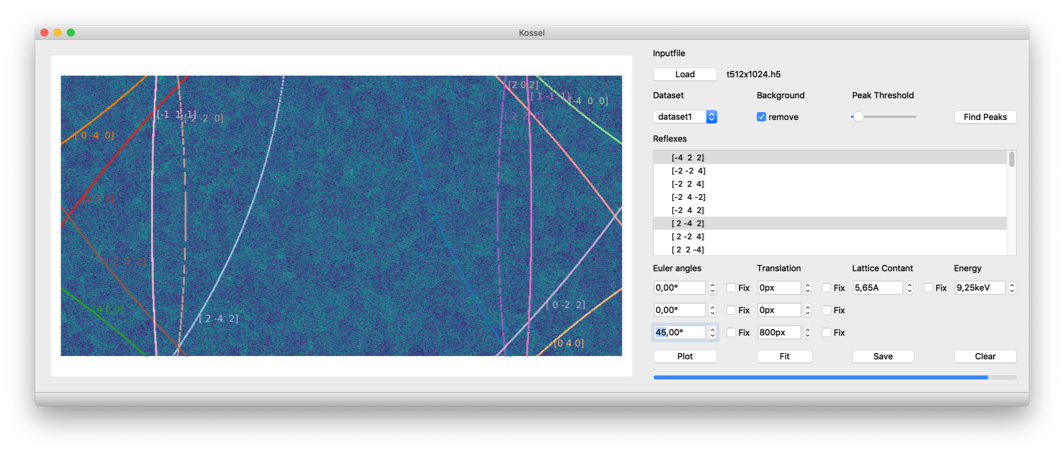
\includegraphics[width=0.8\linewidth]{images/kosselfit.png}
	\caption{Program for fitting Kossel lines to experimental data}
	\label{fig:kosselfit}
\end{figure}




\begin{figure}
	\centering
	\begin{subfigure}{0.35\textwidth}
		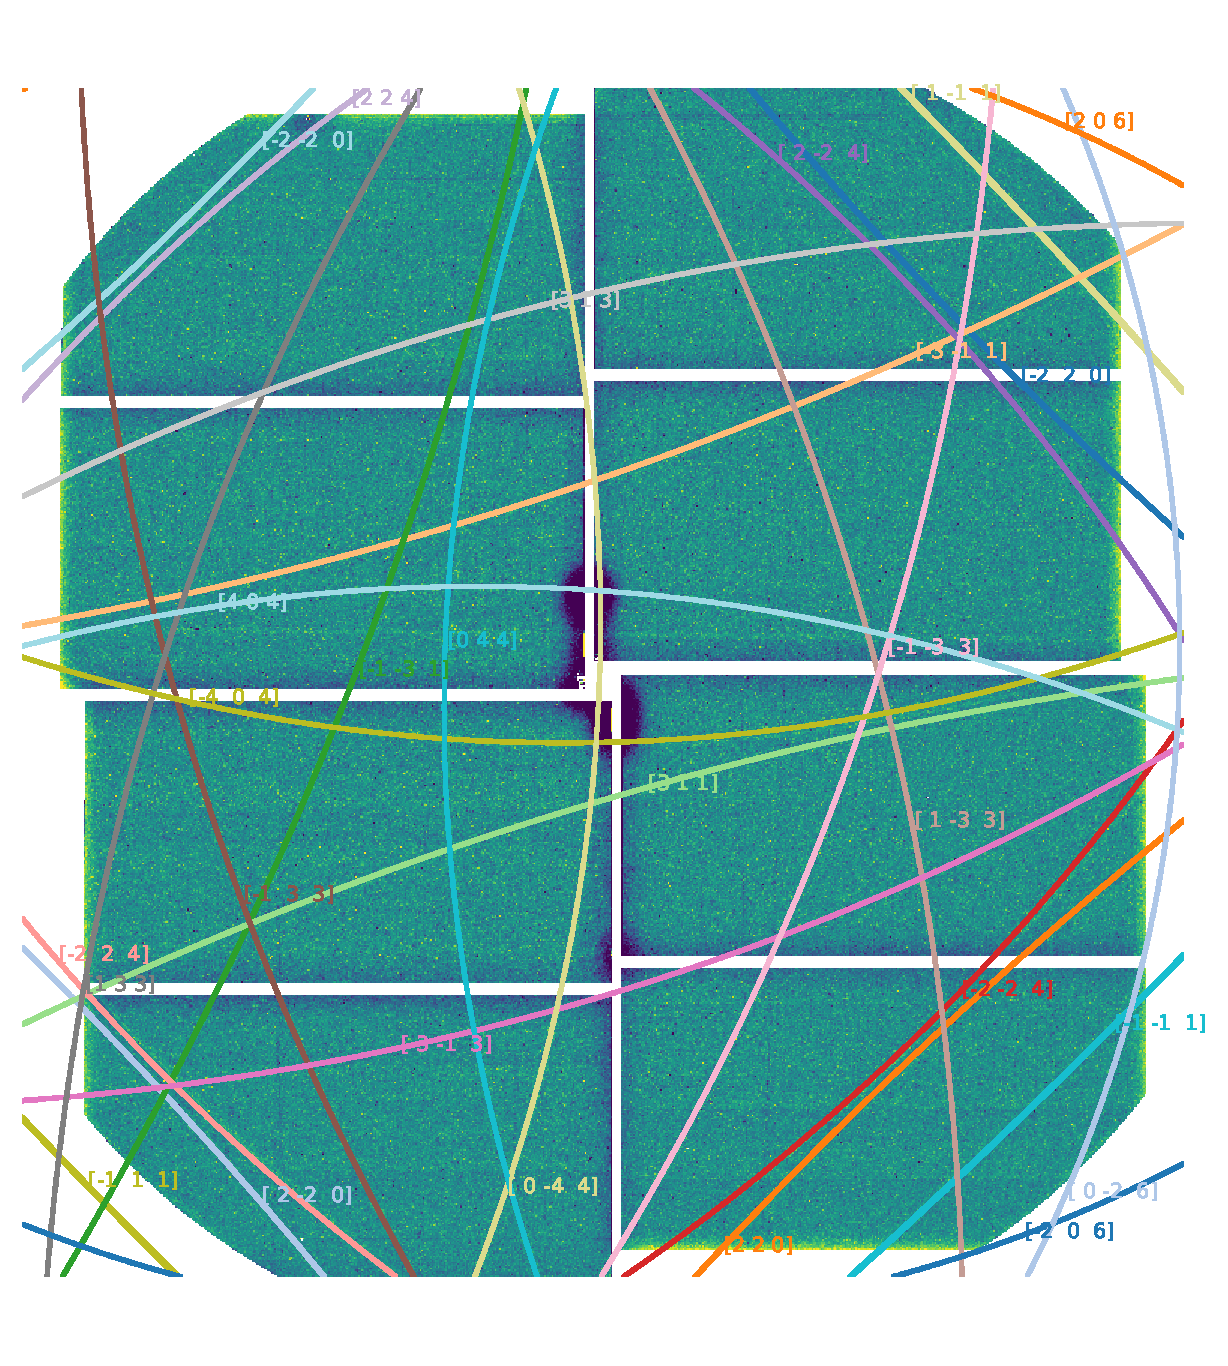
\includegraphics[width=\linewidth]{images/kossel_gaas1.pdf}
		\caption{Indexed lines on sample 1}
	\end{subfigure}
\hspace{0.2cm}
	\begin{subfigure}{0.35\textwidth}
		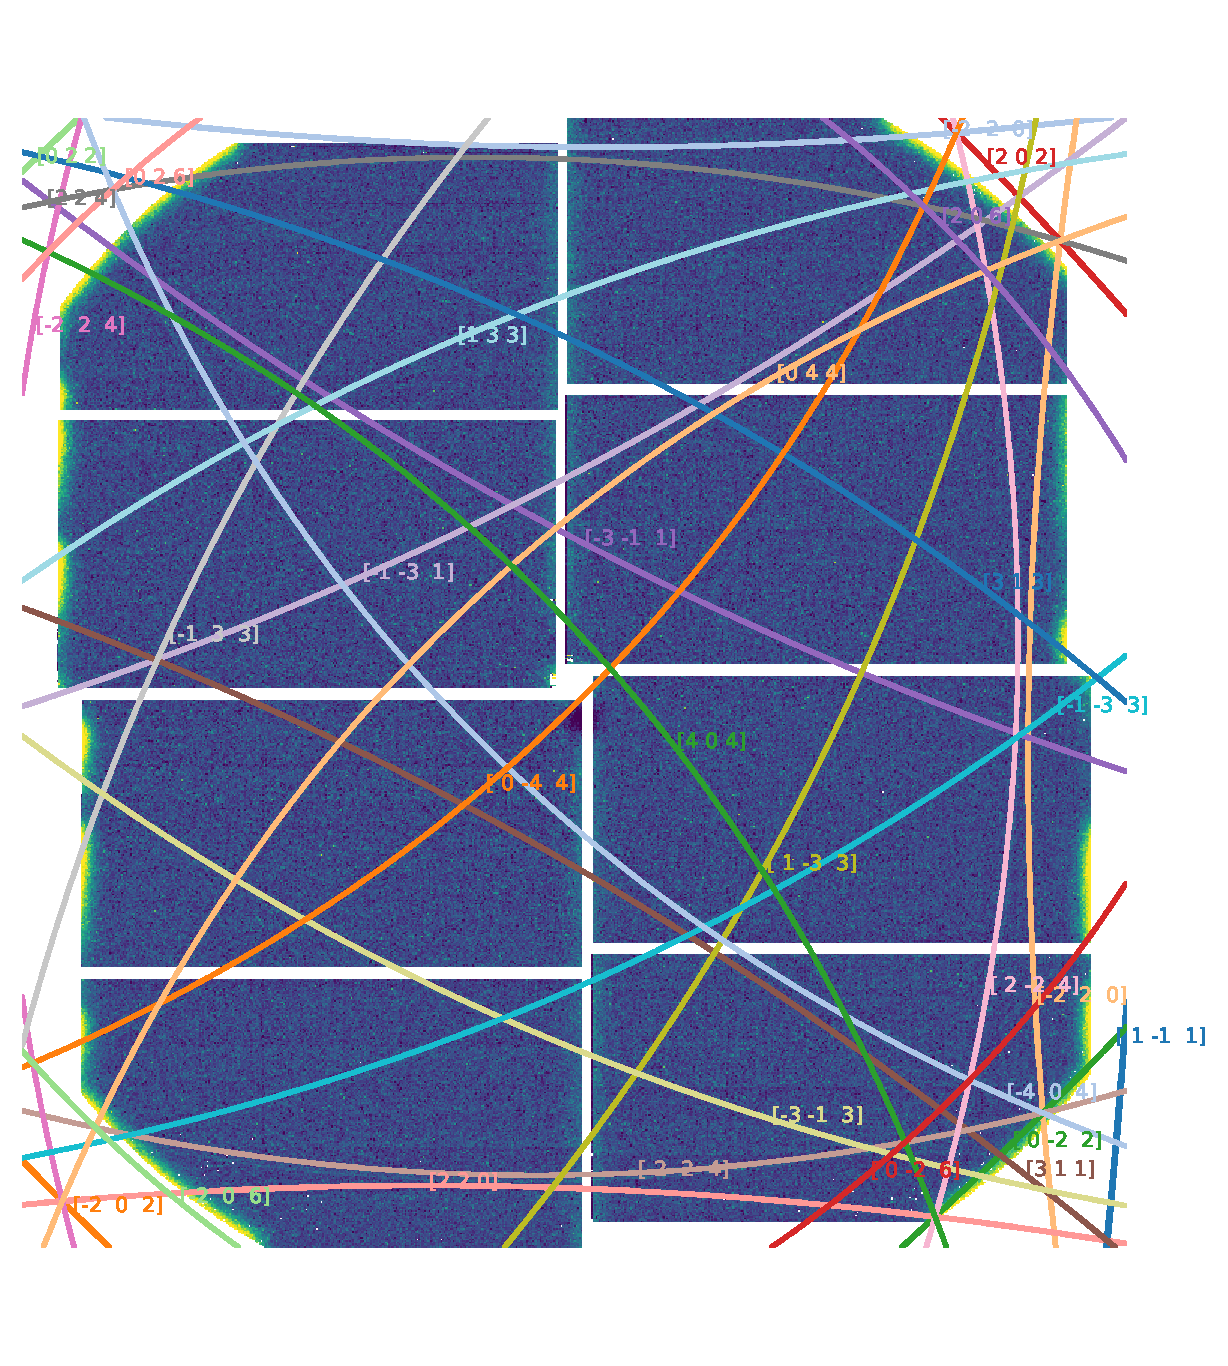
\includegraphics[width=\linewidth]{images/kossel_gaas2.pdf}
		\caption{Indexed lines on sample 2}
	\end{subfigure}
	\caption[Kossel lines on GaAs samples]{Indexed Kossel lines in the determined orientation overlaid over the mean of 5000 shots after background subtraction. For a list of all considered indices, see  \fref{tab:kosselpeaks}.}
	\label{fig:kosselgaasline}
\end{figure}

\begin{table}[]
	\caption{Results of the Kossel line analysis}
\begin{tabular}{llllllll}
	\hline
	Sample & \multicolumn{2}{l}{Translation} & \multicolumn{3}{l}{Rotation}  & Detector Distance &  \\
	& x in mm        & y in mm        & yaw              & pitch           & roll           & in mm             &  \\ 
	\hline
	GaAs 1 & 1.4$\pm$0.2    & 6.4$\pm$0.4    & -0.4°$\pm$0.2° & 0.1°$\pm$0.2° & 1.5°$\pm$0.2° & 141.7$\pm$0.8     &  \\
	GaAs 2 & 1.3$\pm$0.2    & 5.8$\pm$0.3    & -0.2°$\pm$0.3° & 0.1°$\pm$0.2° & 46.1°$\pm$0.1° & 139.9$\pm$0.8     &  \\
	\hline
\end{tabular}
	
	\label{tab:kosselfit}
\end{table}

\subsection{Reconstruction}
For the foil data, the small angle approximation is valid and each pixel can be thought of as having the same XXX angle, permitting using the pixelwise correlation as a reconstruction.

For the nanoparticle data, detection angle is higher and therefor the $\delta q$ is lower for pixels further of axis. Therefor, for each pixel the $q$ value is calculated and a radial correlation with the corrected values is performed.

For the crystal data, a full 3d correlation in $q$ space is performed.


\section{Results}
\subsection{Imaging the Focus}

The reconstruction if performed once without discretization and only applying a threshold of 1500\,eV and once with discretization into photons. 




The excited volume can in the horizontal direction be approximated as a rectangular function with a width of $\sqrt{2}$-times the thickness of the foil used, due to the 45° angle, if the (horizontal) FWHM of the focus is much smaller than the thickness of the foil and ignoring absorption.  In the vertical direction, the volume is limited by the (vertical) FWHM of the focus and can be (roughly) approximated to be Gaussian. 
In the small angle approximation, the reconstruction is the magnitude squared of the 2D Fourier transform of the volume (see XXX). As the magnitude squared of the Fourier transform of a Gaussian with FWHM $f$ is another Gaussian with FWHM $\frac{4\sqrt{2}\log{2}}{f}$ and the magnitude squared of the Fourier transform of a rectangular function with width $w$ is proportional to $\sinc^2{\left(\frac{q w}{2}\right)}$
\footnote{If the foil were thicker, the absorption length $a$ could not be ignored and the more complicated $\left|\mathscr{F}\left(e^{-\frac{x}{a}} \Pi \left(\frac{x}{w}\right)\right)\right|^2 \propto \frac{\cosh \left(\frac{w}{a}\right)-\cos (q w)}{a^2 q^2+1}$
 could be used instead.}, a 2D least-squares regression of the product of those functions is performed with the reconstructed image to estimate the focal FWHM \cite{butz2015}. As the horizontal direction is under sampled, the horizontal profile will not be resolved in the reconstruction. To account for the binning in the reconstruction, the function used for the regression is sampled at 25x the resolution in both directions and averaged (corresponding to a convolution with an rectangular sampling kernel). 
\subsubsection{Filtering}

\subsection{Imaging Nanoparticles}
\subsubsection{Filtering}
\subsection{Imaging Crystals}




